\documentclass[11pt,a4paper]{article}

% ---------- Codificación y fuentes ----------
\usepackage[utf8]{inputenc}
\usepackage[T1]{fontenc}
\usepackage{lmodern}
\usepackage[spanish,es-nodecimaldot]{babel}
\usepackage{microtype}

% ---------- Geometría ----------
\usepackage[a4paper,top=2.6cm,bottom=2.4cm,left=2.3cm,right=2.3cm,headheight=22pt,headsep=0.7cm,footskip=1.1cm]{geometry}

% ---------- Paquetes ----------
\usepackage{amsmath,amssymb}
\usepackage{graphicx}
\usepackage{xcolor}
\usepackage{booktabs}
\usepackage{array}
\usepackage{tabularx}
\usepackage{enumitem}
\usepackage{float}
\usepackage{caption}
\usepackage{fancyhdr}
\usepackage{titlesec}
\usepackage{lastpage}
\usepackage{needspace}
\usepackage{siunitx}
\usepackage{pgfgantt}
\usepackage{listings}
\usepackage[hidelinks]{hyperref}
\usepackage{tikz}
\usepackage[european,straightvoltages]{circuitikz}
\usetikzlibrary{babel,positioning,arrows.meta,calc,automata,fit,backgrounds}
\graphicspath{{figuras/}{../plan/}{../fotos/}}

\sisetup{output-decimal-marker={,}, per-mode=symbol}

% ---------- Colores ----------
\definecolor{navy}{HTML}{17365D}
\definecolor{blue}{HTML}{1F4E79}
\definecolor{accent}{HTML}{2E5C8A}
\definecolor{softblue}{HTML}{DCE6F1}
\definecolor{softgreen}{HTML}{E2EFDA}
\definecolor{softorange}{HTML}{FCE4D6}
\definecolor{graytext}{HTML}{595959}

% ---------- Estilo general ----------
\setlength{\parindent}{0pt}
\setlength{\parskip}{5pt}
\renewcommand{\baselinestretch}{1.04}

% ---------- Títulos ----------
\titleformat{\section}
  {\Needspace{12\baselineskip}\Large\bfseries\color{navy}}{\thesection.}{0.55em}{}
  [\vspace{2pt}{\color{accent}\rule{\linewidth}{0.6pt}}]
\titlespacing*{\section}{0pt}{14pt}{6pt}

\titleformat{\subsection}
  {\Needspace{8\baselineskip}\large\bfseries\color{accent}}{\thesubsection}{0.5em}{}
\titlespacing*{\subsection}{0pt}{10pt}{3pt}

\titleformat{\subsubsection}
  {\normalsize\bfseries\color{accent}}{\thesubsubsection}{0.5em}{}
\titlespacing*{\subsubsection}{0pt}{8pt}{2pt}

% ---------- Cabeceras y pies ----------
\pagestyle{fancy}
\fancyhf{}
\fancyhead[L]{\small\color{accent}Trabajo final · Informe}
\fancyhead[R]{\small\color{accent}Sistemas Digitales}
\renewcommand{\headrulewidth}{0.4pt}
\renewcommand{\headrule}{\hbox to\headwidth{\color{accent}\leaders\hrule height \headrulewidth\hfill}}
\fancyfoot[C]{\small\color{accent}\thepage/\pageref{LastPage}}

% ---------- Captions ----------
\captionsetup[table]{name=Tabla}
\captionsetup{
  font=small,
  labelfont={bf,color=navy},
  labelsep=colon,
  justification=justified,
  skip=4pt
}

% ---------- Código ----------
\lstset{
  basicstyle=\ttfamily\footnotesize,
  keywordstyle=\color{navy}\bfseries,
  commentstyle=\color{graytext}\itshape,
  backgroundcolor=\color{softblue!40},
  frame=single, rulecolor=\color{accent!50},
  framesep=4pt, xleftmargin=6pt, xrightmargin=6pt,
  columns=fullflexible, keepspaces=true,
  literate={á}{{\'a}}1 {é}{{\'e}}1 {í}{{\'i}}1 {ó}{{\'o}}1 {ú}{{\'u}}1 {ñ}{{\~n}}1
}

% ---------- TikZ ----------
\tikzset{
  block/.style={draw=navy, fill=softblue, rounded corners=2pt, minimum width=2.2cm,
    minimum height=1.0cm, align=center, font=\small, inner sep=3pt},
  pcblock/.style={block, fill=softgreen},
  hwblock/.style={block, fill=softorange},
  arr/.style={-{Latex[length=2mm]}, draw=navy, thick},
  lab/.style={font=\scriptsize, color=graytext}
}

\begin{document}

% ======================================================================
% PORTADA
% ======================================================================
\begin{titlepage}
\thispagestyle{empty}

\noindent\colorbox{navy}{%
  \parbox{\dimexpr\textwidth-2\fboxsep\relax}{%
    \color{white}\sffamily\small
    UNIVERSIDAD DE ZARAGOZA · FACULTAD DE CIENCIAS\\[2pt]
    GRADO EN FÍSICA · SISTEMAS DIGITALES · CURSO 2026/2027}}

\vspace{3.2cm}

{\color{accent}\rule{\textwidth}{0.6pt}}

\vspace{0.75cm}
{\color{navy}\bfseries\fontsize{30}{34}\selectfont Trabajo final\par}
\vspace{0.25cm}
{\color{accent}\sffamily\fontsize{17}{21}\selectfont
Sistema de lectura del pulso cardiaco\par}
\vspace{0.35cm}
{\color{graytext}\fontsize{11}{14}\selectfont
Informe: pulsómetro por fotopletismografía con Arduino Nano. Frecuencia cardiaca,
variabilidad (HRV), indicador de estado y visualización en tiempo real\par}
\vspace{0.55cm}
{\color{accent}\rule{\textwidth}{0.6pt}}

\vspace{1.7cm}

\begin{center}
\renewcommand{\arraystretch}{1.9}
\begin{tabular}{r@{\hspace{0.6em}}p{8.4cm}}
\textbf{Autores:} & \rule{8.4cm}{0.4pt}\\[-4pt]
                  & \rule{8.4cm}{0.4pt}\\[2pt]
\textbf{Fecha:}   & noviembre de 2026\\
\end{tabular}
\end{center}

\vfill
{\color{graytext}\small
\raggedright
Código, grabaciones y notas de cada módulo en la carpeta del trabajo: \texttt{firmware/},
\texttt{pc/}, \texttt{datos/} e \texttt{informe/}. El plan de desarrollo
(\texttt{plan/}) detalla el procedimiento de cada módulo.\par}

\end{titlepage}

\setcounter{page}{1}
\tableofcontents
\newpage

% ======================================================================
\section{Objetivos y resultado}

El objetivo es un sistema basado en Arduino Nano que lea el pulso cardiaco por
fotopletismografía (PPG) con el pulsómetro del laboratorio, detecte cada latido y calcule en
tiempo real la frecuencia cardiaca (BPM) y la variabilidad de la frecuencia cardiaca (HRV:
RMSSD y SDNN). Como ampliaciones: un indicador de estado \{relajado, normal, estrés\} y la
representación de la onda en tiempo real en el PC.

El trabajo se dividió en módulos independientes (M0 a M9), cada uno con su prueba de
verificación, de forma que siempre hubiera una versión funcional. La Tabla~\ref{tab:resultado}
resume los criterios que se fijaron al principio y lo conseguido.

\begin{table}[H]
\centering\small
\caption{Criterios de éxito del plan y resultado.}
\label{tab:resultado}
\begin{tabularx}{\textwidth}{lXX}
\toprule
Funcionalidad & Criterio & Resultado \\
\midrule
Adquisición & \qty{500}{Hz} por interrupción, sin pérdidas & \qty{500.39}{Hz}; 0 muestras perdidas en todas las sesiones \\
Detección de latidos & Sin latidos perdidos ni duplicados en reposo & 89 latidos en \qty{60}{s}, igual que un contador de picos independiente; 0 rechazos en \qty{39}{s} de reposo \\
BPM & Error $\le \qty{2}{BPM}$ frente a una referencia & 77,6 frente a \qty{79}{BPM} de una app de móvil: \qty{1.4}{BPM} \\
HRV & Error $\le \qty{2}{ms}$ con RR conocidos & RMSSD 100,9 y SDNN \qty{51.4}{ms} (esperado 100 y 50,9) \\
Onda en tiempo real & $\ge 20$ fps, sin retraso acumulado & 20-\qty{25}{fps}, retraso estable de unos ms \\
Indicador de estado & Tendencia esperada en el protocolo & Estrés \qty{10}{s} después de empezar la prueba de prensión; relajado con respiración lenta; probado con dos personas \\
LCD y LED RGB & Funcionamiento sin PC & No se hizo (opcional) \\
\bottomrule
\end{tabularx}
\end{table}

% ======================================================================
\section{Fundamento}

\textbf{Fotopletismografía.} La sangre absorbe luz mucho más que el tejido que la rodea. En
cada sístole aumenta el volumen de sangre arterial en el dedo y llega menos luz al detector.
La intensidad tiene una componente casi constante (tejido, hueso, sangre venosa) y una
pulsátil de un pequeño porcentaje, sincronizada con el latido. La señal útil es, por tanto,
una variación de milivoltios sobre un nivel de voltios: hay que quitar la continua y
amplificar.

\textbf{Frecuencia cardiaca y HRV.} Del instante de cada latido se obtienen los intervalos
entre latidos ($RR_i$, en ms). Para $N$ intervalos:
\begin{gather*}
  \mathrm{BPM} = \frac{60000}{\overline{RR}}, \\
  \mathrm{SDNN} = \sqrt{\frac{1}{N-1}\sum_{i=1}^{N}\left(RR_i - \overline{RR}\right)^2},
  \qquad
  \mathrm{RMSSD} = \sqrt{\frac{1}{N-1}\sum_{i=1}^{N-1}\left(RR_{i+1} - RR_i\right)^2}.
\end{gather*}
SDNN mide la variabilidad global y RMSSD la variabilidad latido a latido, ligada a la
actividad parasimpática (vagal). Un corazón sano no late como un metrónomo: con la
respiración el ritmo se acelera al inspirar y se frena al espirar (arritmia sinusal
respiratoria), y esa es la variación que se mide. Con PPG se obtiene en rigor la variabilidad
del \emph{pulso} (PRV), que en reposo coincide bien con la del ECG~[5].

% ======================================================================
\section{Arquitectura}

\begin{figure}[H]
\centering
\begin{tikzpicture}[node distance=0.55cm and 0.55cm, font=\small]
  \node[block] (adc) {ADC + Timer1\\\qty{500}{Hz}\\\scriptsize M3};
  \node[block, left=of adc] (det) {Detector de\\latidos, RR\\\scriptsize M5};
  \node[block, left=of det] (hrv) {BPM, HRV\\\scriptsize M6};
  \node[block, left=of hrv] (est) {Estado\\\scriptsize M7};
  \node[block, left=of est] (out) {Protocolo\\serie, EEPROM};
  \node[hwblock, above=1.3cm of adc] (acon) {Acondicionamiento\\TL082 \qty{\pm 12}{V}\\\scriptsize M2};
  \node[hwblock, left=of acon] (exc) {Divisor\\con LDR\\\scriptsize M1};
  \node[hwblock, left=of exc] (sen) {LED blanco\\+ LDR\\\scriptsize M0};
  \node[pcblock, below=1.1cm of out] (pc) {Visor\\\scriptsize M4};
  \node[pcblock, right=of pc] (an) {Análisis\\y banco de pruebas\\\scriptsize M9};

  \draw[arr] (sen) -- (exc);
  \draw[arr] (exc) -- node[above,lab]{$V_s$} (acon);
  \draw[arr] (acon) -- node[right,lab]{A0} (adc);
  \draw[arr] (adc) -- (det);
  \draw[arr] (det) -- (hrv);
  \draw[arr] (hrv) -- (est);
  \draw[arr] (est) -- (out);
  \draw[arr] (out) -- node[left,lab]{USB \qty{115200}{baud}} (pc);
  \draw[arr] (pc) -- node[above,lab]{CSV} (an);

  \begin{scope}[on background layer]
    \node[draw=accent, dashed, rounded corners, inner sep=6pt, fit=(adc)(det)(hrv)(est)(out),
          label={[lab]below right:Arduino Nano (ATmega328P)}] {};
  \end{scope}
\end{tikzpicture}
\caption{Diagrama de bloques. Naranja: hardware analógico; azul: firmware; verde: software en
el PC.}
\label{fig:bloques}
\end{figure}

Todo el procesado se hace en el Arduino: el PC solo visualiza y registra. El muestreo es por
interrupción del Timer1, porque un periodo fijo es imprescindible para medir RR con precisión
de milisegundos. Los módulos de cálculo del firmware (detector, HRV, estado) son C++ sin
dependencias de Arduino, así que el mismo código se compila también en el PC y se prueba con
señales sintéticas y con todas las grabaciones reales antes de cargarlo en el Nano.

% ======================================================================
\Needspace{25\baselineskip}
\section{Hardware}

\subsection{Sensor (M0)}

\begin{figure}[H]
\centering
\begin{minipage}[c]{0.27\textwidth}
  \centering
  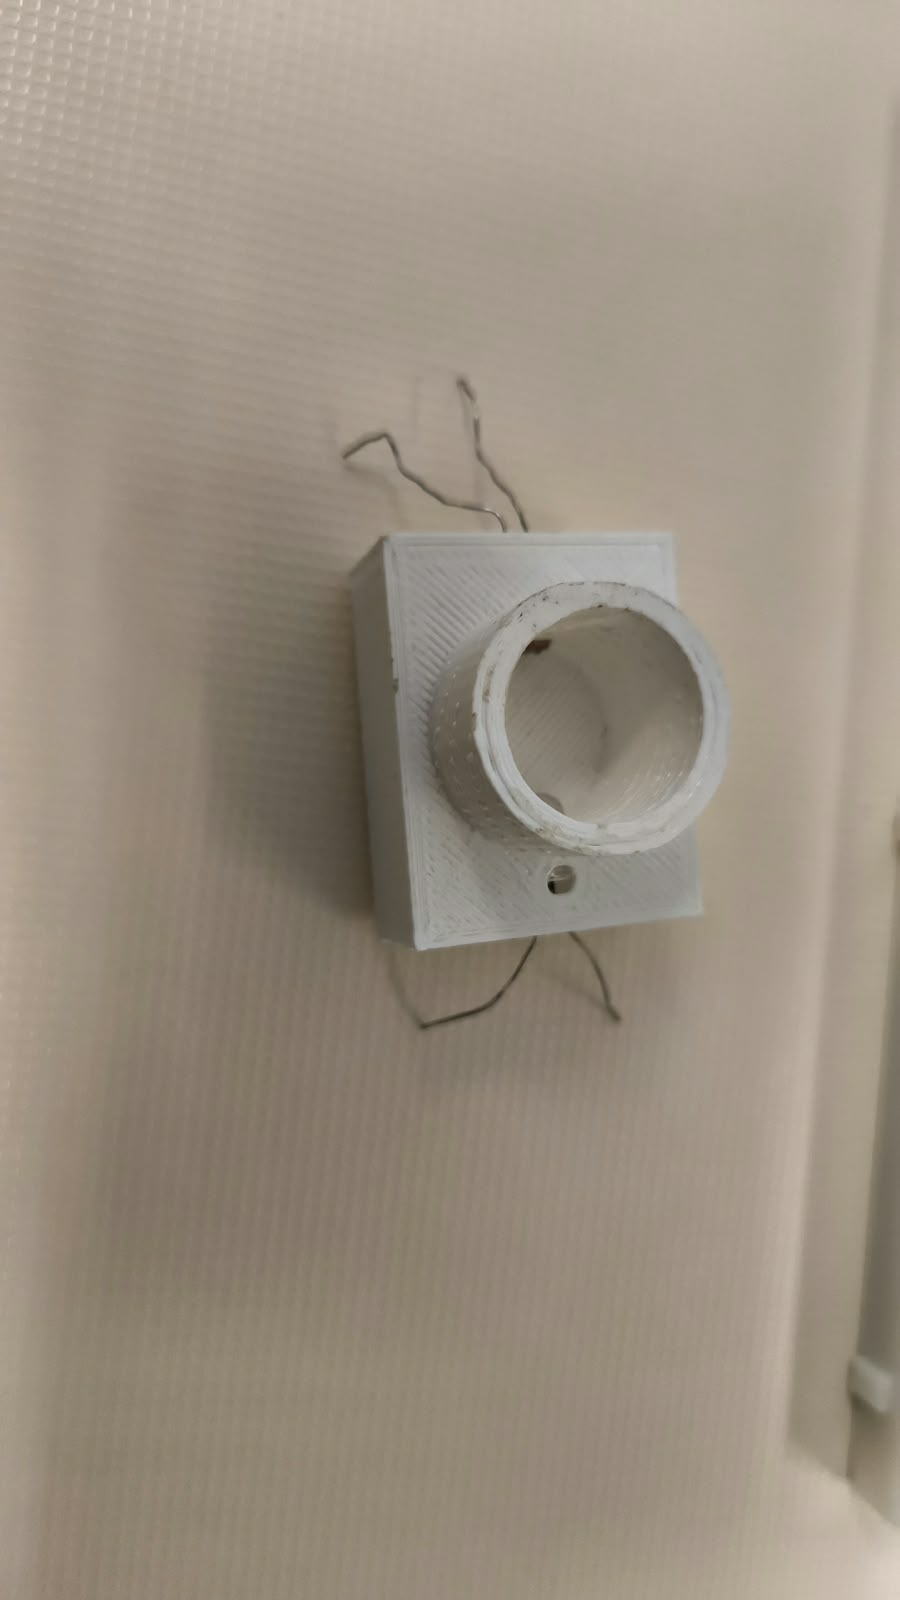
\includegraphics[width=\linewidth,trim=250 400 150 350,clip]{sensor_pulsometro.jpeg}
\end{minipage}\hfill
\begin{minipage}[c]{0.69\textwidth}
\small
\renewcommand{\arraystretch}{1.1}
\begin{tabularx}{\linewidth}{Xr}
\toprule
Situación & $R_{LDR}$ \\
\midrule
Tapada con la mano & $\approx \qty{250}{\kilo\ohm}$ \\
Luz de sala & 10-\qty{90}{\kilo\ohm} \\
LED del sensor apagado (sala) & \qty{13.5}{\kilo\ohm} \\
LED encendido, sin dedo & \qty{0.3}{\kilo\ohm} \\
LED encendido, con dedo & $\approx \qty{4.0}{\kilo\ohm}$ \\
\bottomrule
\end{tabularx}
\end{minipage}
\caption{Pulsómetro del laboratorio (carcasa 3D con cuatro hilos) y resistencia del detector
medida en distintas condiciones.}
\label{fig:sensor}
\end{figure}

El sensor no traía documentación. Con el multímetro: el emisor se enciende pero la prueba de
diodo marca fuera de rango, lo que corresponde a un \textbf{LED blanco} ($V_F \approx
\qty{3}{V}$). El detector no se comporta como un diodo y su resistencia es simétrica y
depende de la luz: es una \textbf{LDR}. La hipótesis inicial del plan (LED infrarrojo y
fototransistor) era incorrecta, y todo el circuito de entrada se diseñó a partir de estas
medidas.

\subsection{Excitación y divisor (M1)}

\begin{figure}[H]
\centering
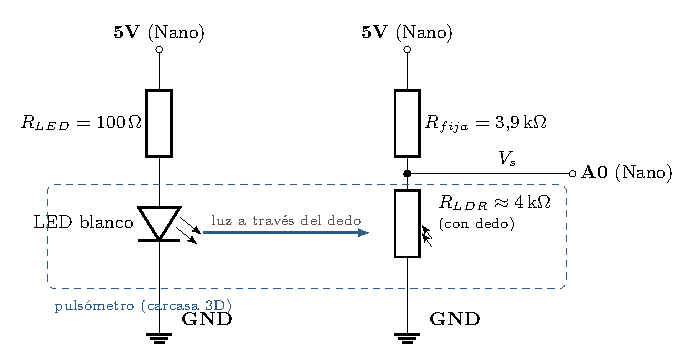
\includegraphics[width=0.6\textwidth]{paso4_divisor_ldr.pdf}
\caption{LED con \qty{100}{\ohm} y divisor con la LDR en la parte baja.}
\label{fig:m1}
\end{figure}

\begin{itemize}[leftmargin=1.2em,itemsep=2pt,topsep=2pt]
  \item \textbf{LED}: $I = (5 - V_F)/R \approx (5 - 3{,}1)/\qty{97.1}{\ohm} \approx
        \qty{19.6}{mA}$, dentro de los \qty{20}{mA} nominales. Se alimenta desde el
        \qty{5}{V} del Nano y no desde un pin, que no debe dar esa corriente de forma
        continua.
  \item \textbf{Resistencia fija}: la sensibilidad del divisor,
        $\partial V_s/\partial R_{LDR} = V_{CC}\,R/(R + R_{LDR})^2$, es máxima con
        $R = R_{LDR}$. Con el dedo $R_{LDR} \approx \qty{4}{\kilo\ohm}$: se elige
        \qty{3.9}{\kilo\ohm} (serie E12), que da el 99,98\,\% de la sensibilidad máxima y deja
        $V_s \approx V_{CC}/2$. El óptimo es muy plano, así que la sensibilidad apenas cambia
        con la presión del dedo.
  \item \textbf{LDR abajo}: más sangre $\Rightarrow$ menos luz $\Rightarrow$ más $R_{LDR}$
        $\Rightarrow$ más $V_s$. El latido sale como un máximo, sin tener que invertir la
        señal.
\end{itemize}

\textbf{Medida} (Figura~\ref{fig:m1senal}): $V_s = \qty{0.37}{V}$ sin dedo y 2,5-\qty{2.7}{V}
con el dedo, como se esperaba. Grabada directamente con el ADC, la componente del pulso mide
solo $\approx \qty{9}{mV}$ p-p: unos 2 escalones del ADC (\qty{4.9}{mV}). En 32 s el
Arduino solo usó 17 valores distintos; el pulso se ve en el espectro (\qty{1.56}{Hz},
\qty{94}{BPM}) pero no latido a latido. Hace falta una ganancia de unas 100 veces.

\begin{figure}[H]
\centering
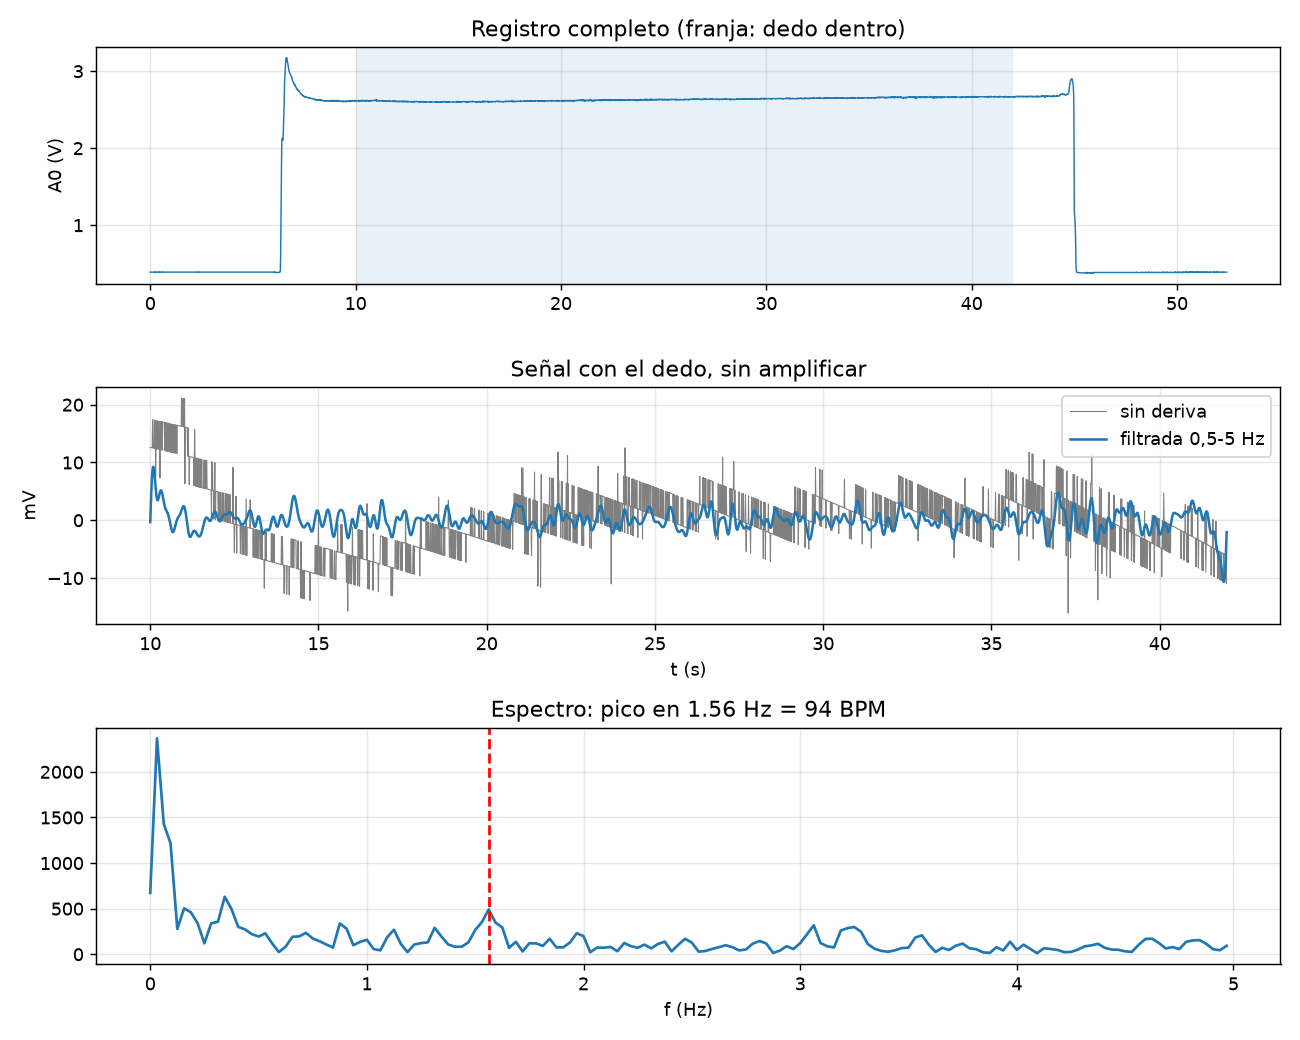
\includegraphics[width=0.85\textwidth]{m1_senal_sin_amplificar.png}
\caption{$V_s$ sin amplificar con el dedo: el pulso queda por debajo de la resolución útil del
ADC.}
\label{fig:m1senal}
\end{figure}

\subsection{Acondicionamiento analógico (M2)}

El único amplificador operacional disponible era el TL082 (doble, entrada JFET). No sirve a
\qty{5}{V}: su entrada en modo común empieza unos \qty{4}{V} por encima de la alimentación
negativa y su salida no se acerca a menos de $\approx\qty{1.5}{V}$ de cada alimentación. Se
alimenta a \qty{\pm 12}{V} con la fuente doble del laboratorio (dos canales en serie, con el
punto común unido al GND del Nano). Así todas las etapas trabajan alrededor de \qty{0}{V} y
no hace falta generar una tensión de referencia. Como la salida podría llegar a
\qty{\pm 10}{V}, al final se desplaza la señal al centro del ADC y se protege la entrada A0.

\begin{figure}[H]
\centering
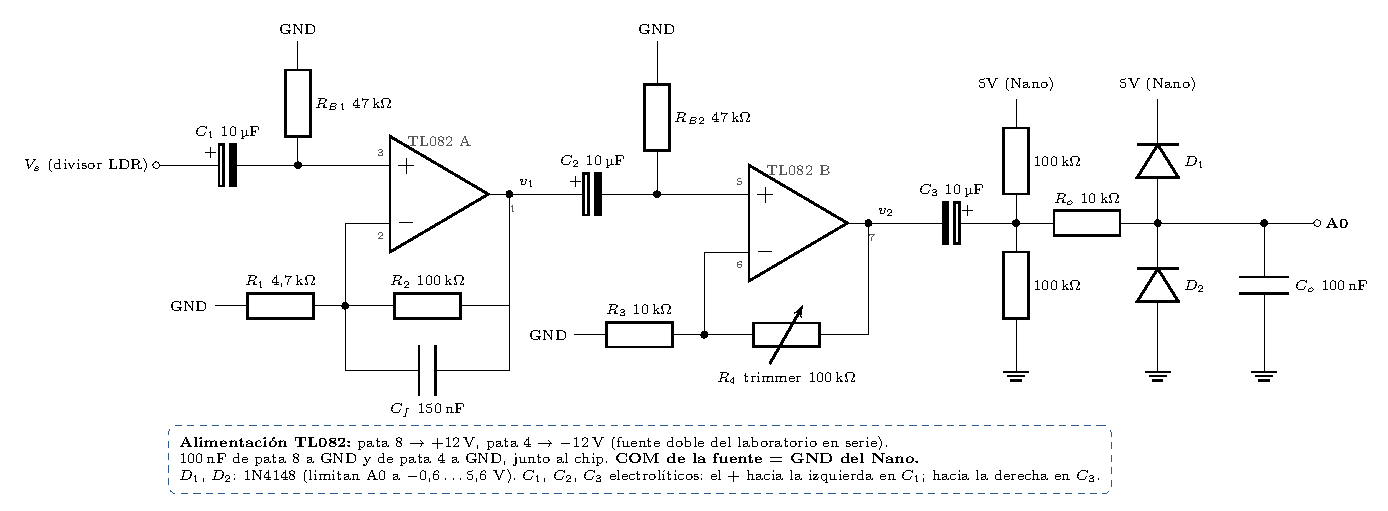
\includegraphics[width=\textwidth]{m2_tl082.pdf}
\caption{Cadena de acondicionamiento construida.}
\label{fig:m2}
\end{figure}

\begin{table}[H]
\centering\small
\caption{Componentes de M2: valor nominal, medido y función.}
\label{tab:m2}
\begin{tabularx}{\textwidth}{llX}
\toprule
Elemento & Medido & Función y cálculo con los valores medidos \\
\midrule
$C_1$, $R_{B1}$ & \qty{10.2}{\micro\farad}, \qty{47.3}{\kilo\ohm} & Paso alto: $1/(2\pi R_{B1}C_1) = \qty{0.33}{Hz}$. Quita la continua de $V_s$ (\qty{2.6}{V}) y la deriva y conserva el pulso (\qtyrange{0.67}{3.3}{Hz}). $R_{B1} \gg$ la salida del divisor: no lo carga. \\
$R_1$, $R_2$ & \qty{4.6}{\kilo\ohm}, \qty{99.2}{\kilo\ohm} & $G_1 = 1 + R_2/R_1 = 22{,}6$. Moderada para que el offset del TL082 (hasta \qty{15}{mV}) no sature. \\
$C_f$ & \qty{147}{\nano\farad} & Paso bajo: $1/(2\pi R_2 C_f) = \qty{10.9}{Hz}$. Conserva la forma del pulso y quita ruido. \\
$C_2$, $R_{B2}$ & \qty{9.34}{\micro\farad}, \qty{46.2}{\kilo\ohm} & Segundo paso alto (\qty{0.37}{Hz}): quita el offset amplificado de la etapa 1. \\
$R_3$, $R_4$ & \qty{9.79}{\kilo\ohm}, \qty{19.9}{\kilo\ohm} & $G_2 = 1 + R_4/R_3 = 3{,}03$; $R_4$ es un potenciómetro de \qty{100}{\kilo\ohm}. \\
$C_3$, $2\times\qty{98.2}{\kilo\ohm}$ & \qty{11.25}{\micro\farad} & Desplaza la señal a la mitad del \qty{5}{V} del Nano. Paso alto de \qty{0.29}{Hz}. \\
$R_o$, $D_1$, $D_2$ & \qty{9.8}{\kilo\ohm}, 1N4148 & Si la etapa satura, los diodos limitan A0 a $-0{,}6\ldots\qty{5.6}{V}$ y $R_o$ limita la corriente. \qty{10}{\kilo\ohm} es la impedancia máxima recomendada para el ADC. \\
$C_o$ & \qty{100}{\nano\farad} & Antialiasing: $1/(2\pi R_o C_o) = \qty{162}{Hz} < f_s/2 = \qty{250}{Hz}$. \\
Desacoplo & 97,1 y \qty{98.9}{\nano\farad} & Patas 8 y 4 del TL082 a GND. \\
\bottomrule
\end{tabularx}
\end{table}

\textbf{Ganancia total}: $G = 22{,}6 \times 3{,}03 = 68{,}5$. La ganancia se reparte en dos
etapas con acoplamiento en alterna entre ellas: el offset de la etapa 1 multiplicado por 68
llevaría la salida hasta \qty{1}{V}, y el segundo paso alto lo elimina antes de la ganancia
final.

\textbf{Punto de trabajo del ADC.} El nodo de salida y A0 miden \qty{2.35}{V}, no
\qty{2.5}{V}: el \qty{5}{V} del Nano alimentado por USB es \qty{4.7}{V} (pasa por un diodo de
protección). El ADC usa esa misma tensión como referencia, así que \qty{2.35}{V} es justo el
centro de escala (ADC $\approx 512$) sea cual sea la tensión del USB.

\textbf{Puesta a punto.}
\begin{itemize}[leftmargin=1.2em,itemsep=2pt,topsep=2pt]
  \item Al principio la etapa 2 saturaba a \qty{+11.2}{V} y el raíl negativo caía a
        \qty{-9}{V} con oscilaciones: faltaba $R_4$ y el amplificador estaba en lazo abierto.
        Además se habían medido resistencias con la fuente encendida, lo que falsea la medida.
        Se corrigió con el potenciómetro y se adoptó la regla de medir resistencias siempre
        sin alimentación.
  \item Con $G_2 = 1$ el pulso medía 0,5-\qty{0.6}{V} p-p en A0. Se ajustó $G_2 = 3{,}03$
        para llegar a 1,5-\qty{2}{V} p-p (Figura~\ref{fig:m2senal}), con margen frente a
        \qty{0}{V} y \qty{4.7}{V} por si el pulso crece con la presión del dedo.
  \item Sin dedo el ruido es de 1 LSB (\qty{5}{mV}): por debajo de la resolución del ADC.
  \item Al meter o sacar el dedo la cadena satura unos \qty{8}{s}, hasta que se cargan
        $C_1$-$C_3$. Es el precio de la ganancia; el firmware lo detecta y reaprende.
  \item El circuito también funciona a \qty{\pm 5}{V}, porque todas las señales están cerca de
        \qty{0}{V}; se mantiene \qty{\pm 12}{V}, donde el fabricante garantiza sus
        características.
\end{itemize}

\begin{figure}[H]
\centering
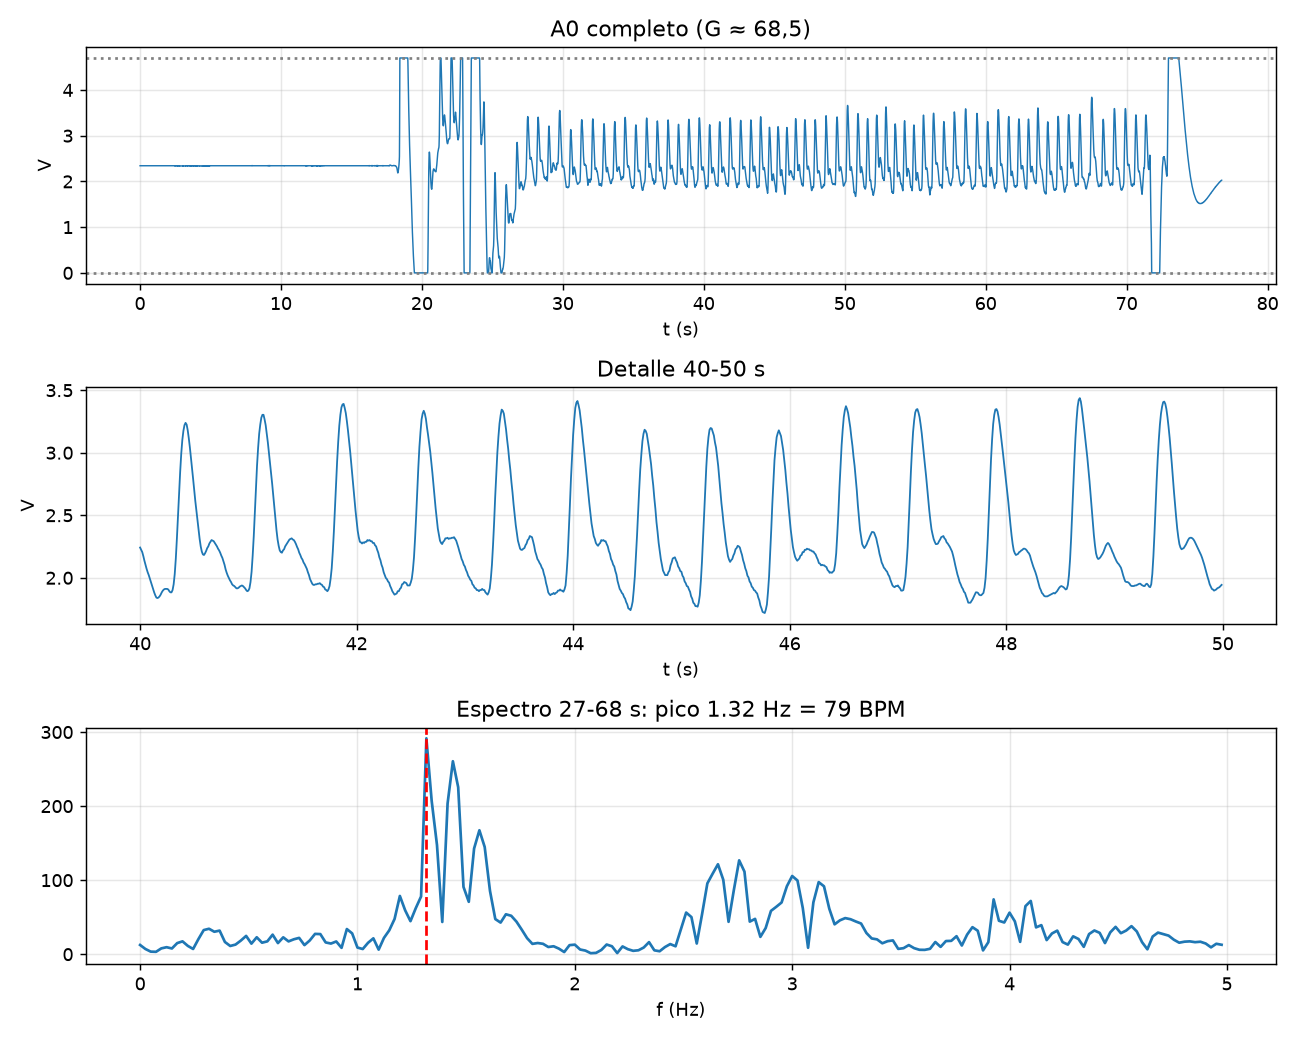
\includegraphics[width=0.85\textwidth]{m2_senal_g68.png}
\caption{Señal en A0 con $G = 68{,}5$: pulso de 1,5-\qty{2}{V} p-p con la muesca dícrota bien
visible, y saturación al meter y sacar el dedo.}
\label{fig:m2senal}
\end{figure}

\subsection{Montaje final}

El circuito completo cabe en una placa de prototipos (Figura~\ref{fig:montaje}): a la
izquierda el TL082 con el potenciómetro de la etapa 2, en el centro el sensor (el LED queda
dentro de la pieza blanca y la LDR debajo del dedo) y a la derecha el Arduino Nano, conectado
al portátil por USB. La fuente doble da \qty{\pm 12}{V} al operacional con su común unido a la
masa del Nano.

\begin{figure}[H]
\centering
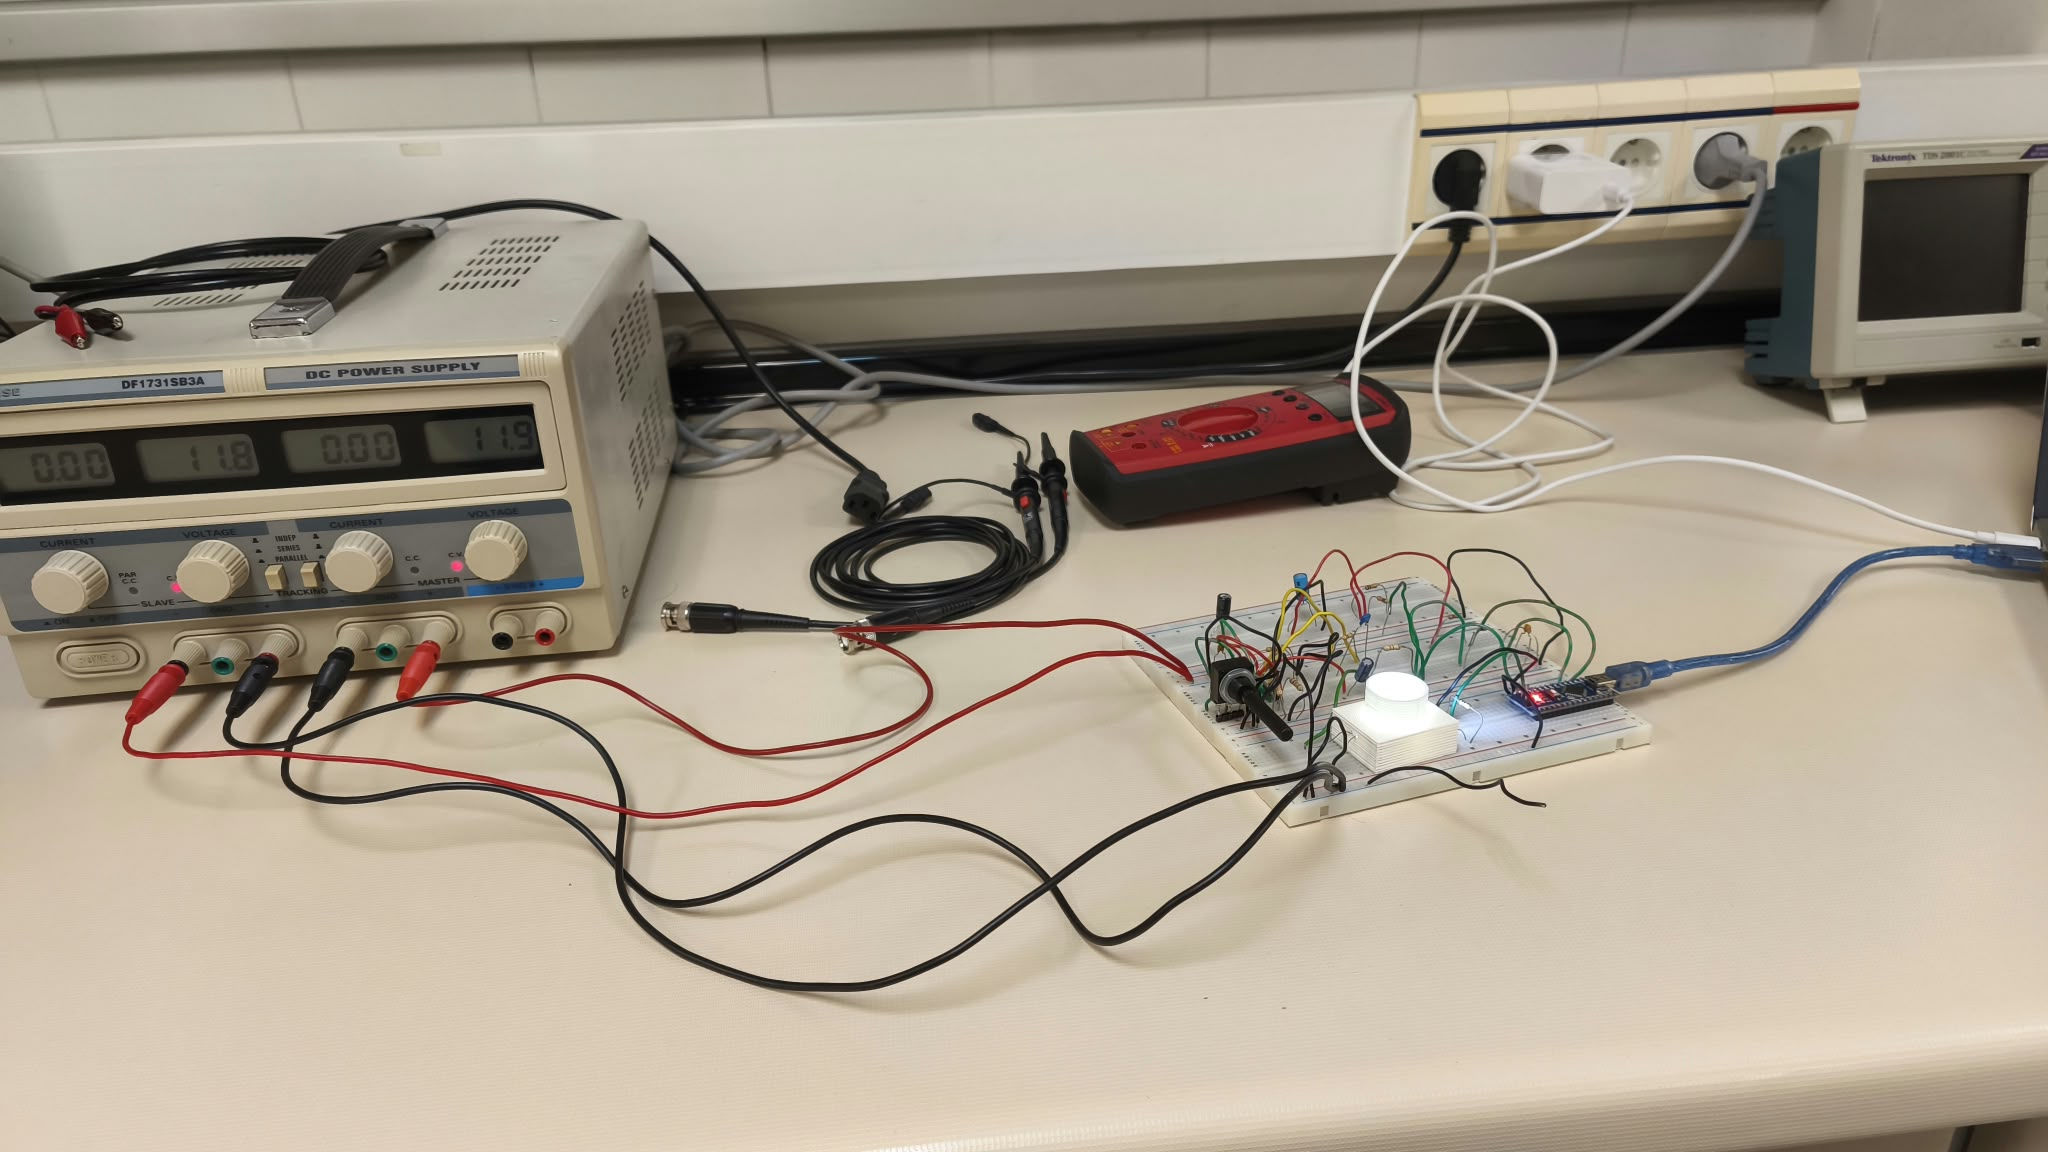
\includegraphics[width=\textwidth]{montaje_fuente.jpg}\\[4pt]
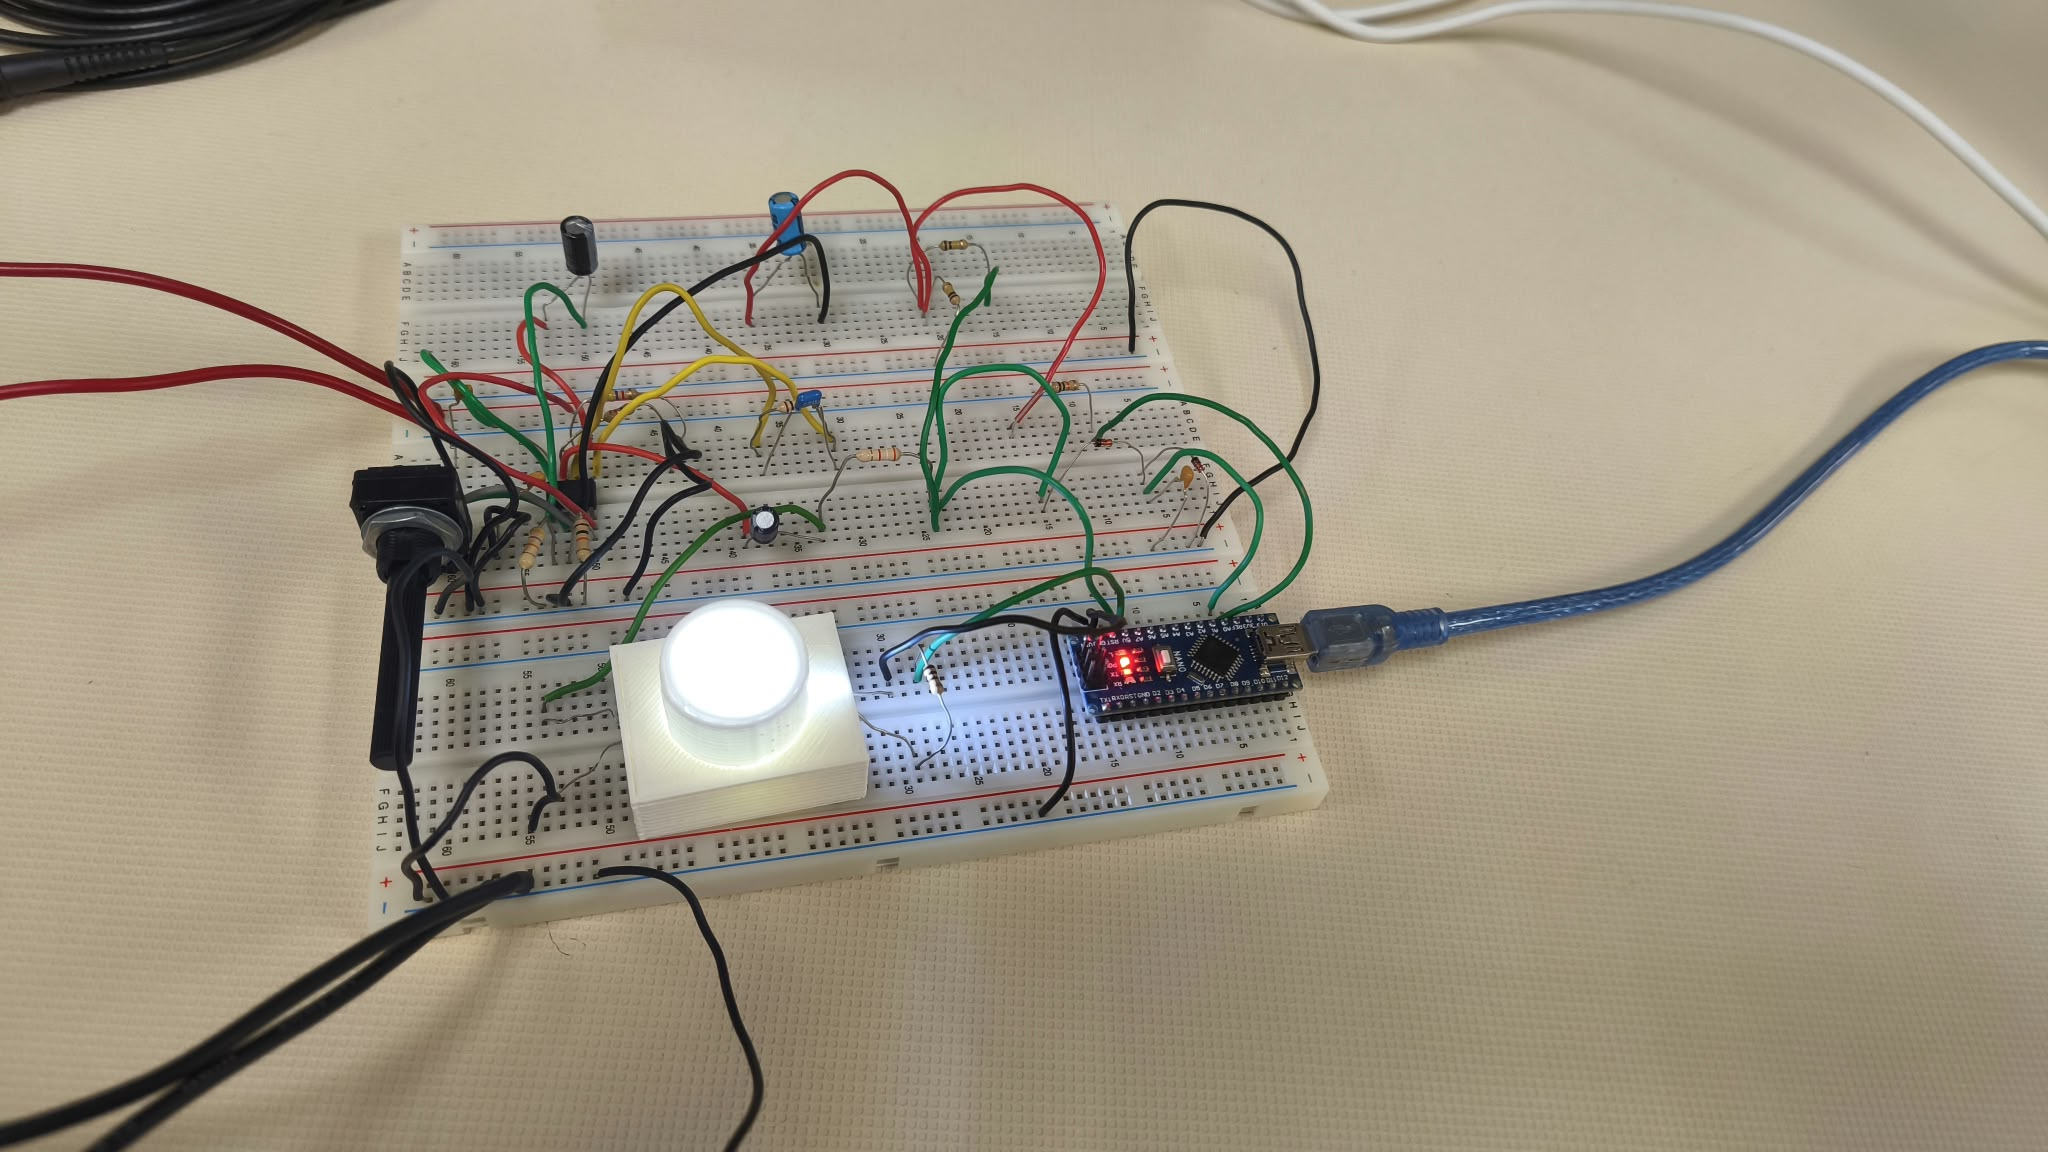
\includegraphics[width=0.495\textwidth]{placa_sin_dedo.jpg}\hfill
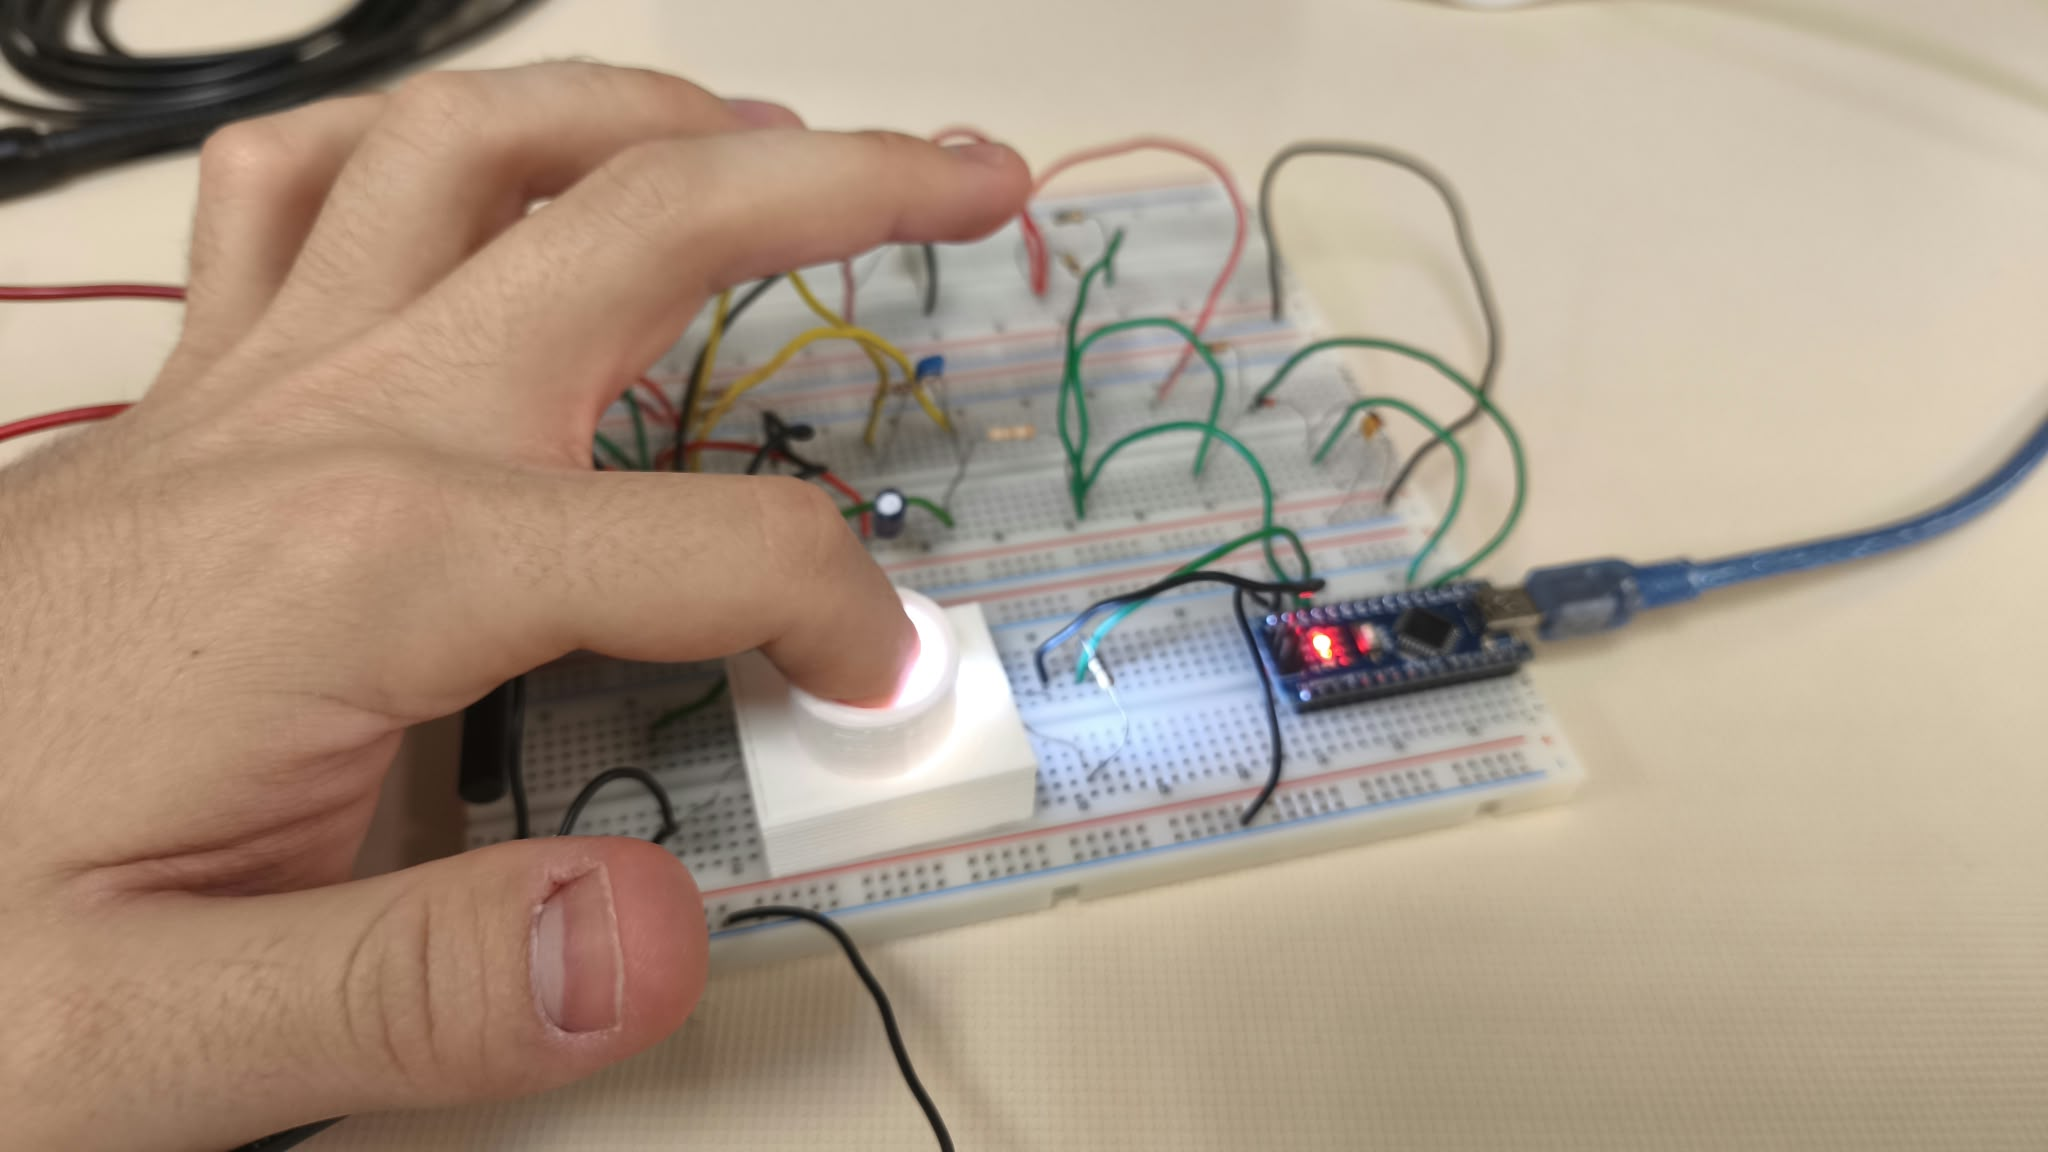
\includegraphics[width=0.495\textwidth]{sensor_con_dedo.jpg}
\caption{Montaje final. Arriba: fuente de \qty{\pm 12}{V} (11,8 y \qty{11.9}{V}), placa y
Nano conectado al portátil. Abajo: la placa sin dedo y midiendo con el dedo sobre el sensor.}
\label{fig:montaje}
\end{figure}

% ======================================================================
\section{Firmware}

El sketch (\texttt{firmware/pulso/}) tiene cuatro módulos: \texttt{adquisicion},
\texttt{detector}, \texttt{hrv} y \texttt{estado}, más \texttt{pulso.ino}, que los
orquesta, implementa el protocolo serie y guarda la línea base en la EEPROM. Ocupa
\qty{11134}{B} de flash (36\,\%) y \qty{1015}{B} de RAM (49\,\%).

\subsection{Adquisición (M3)}

El Timer1 en modo CTC genera una interrupción cada \qty{2}{ms}:
\[
  f_s = \frac{f_{clk}}{N\,(1 + \mathrm{OCR1A})} = \frac{\qty{16}{MHz}}{64\cdot(1 + 499)} =
  \qty{500}{Hz}.
\]
La ISR solo lee A0 y guarda la muestra en un buffer circular de 256 muestras
(\qty{512}{B}, $\approx\qty{0.5}{s}$ de margen); \texttt{loop()} las procesa. Si
\texttt{loop()} se retrasara más que el buffer, las muestras perdidas se cuentan y el detector
se reinicia, porque un RR con un hueco no sería fiable. Al PC se envía una muestra de cada
cinco (\qty{100}{Hz}): todas en ASCII no caben con holgura en \qty{115200}{baud}, y
\qty{100}{Hz} sobra para dibujar una señal de banda \qty{11}{Hz}.

\textbf{Resultado}: \qty{500.39}{Hz} medidos con el reloj del PC (+0,08\,\%, la tolerancia
del oscilador del clon, que da un error de \qty{0.6}{ms} en un RR de \qty{800}{ms}). Cero
muestras perdidas en todas las pruebas, también con el firmware completo enviando datos.

\subsection{Detección de latidos (M5)}

Por cada muestra:
\begin{enumerate}[leftmargin=1.4em,itemsep=2pt,topsep=2pt]
  \item \textbf{Media móvil de 10 muestras.} A \qty{500}{Hz} dura \qty{20}{ms}, un periodo de
        red: su respuesta tiene ceros en \qty{50}{Hz} y sus múltiplos. Una suma y una resta
        por muestra.
  \item \textbf{Umbral adaptativo}: $u = v + 0{,}6\,(p - v)$, con $p$ y $v$ medias
        exponenciales ($\alpha = 0{,}25$) del pico y del valle de cada latido aceptado.
  \item \textbf{Máquina de estados} (Figura~\ref{fig:fsm}). Un latido exige cruzar el umbral
        hacia arriba, una amplitud mínima (\qty{22}{LSB} $\approx \qty{0.1}{V}$) y una relativa
        (40\,\% de la media), y que el RR sea de al menos \qty{300}{ms}. Tras cada latido, un
        periodo refractario del 60\,\% del RR medio, entre 250 y \qty{500}{ms}, tapa la onda
        dícrota.
  \item \textbf{Instante del latido}: punto de máxima pendiente de subida (ver abajo).
\end{enumerate}

\begin{figure}[H]
\centering
\begin{tikzpicture}[shorten >=1pt, node distance=3.6cm, on grid, auto, font=\small,
                    every state/.style={draw=navy, fill=softblue, thick, minimum size=1.75cm, align=center, font=\scriptsize}]
  \node[state, initial, initial text={}] (A) {APRENDI-\\ZAJE};
  \node[state, right=of A] (E) {ESPERA};
  \node[state, right=of E] (S) {SUBIDA};
  \node[state, right=of S] (R) {REFRAC-\\TARIO};
  \path[arr]
    (A) edge node[above, font=\scriptsize]{\qty{2}{s}} (E)
    (E) edge node[above, align=center, font=\scriptsize]{cruce de\\subida de $u$} (S)
    (S) edge node[above, align=center, font=\scriptsize]{$y < u$, latido\\válido: RR} (R)
    (S) edge[bend left=40] node[below, font=\scriptsize]{pico no válido} (E)
    (R) edge[bend left=45] node[below, align=center, font=\scriptsize]{$t - t_{pico} > $ refractario} (E)
    (E) edge[bend right=45] node[above, align=center, font=\scriptsize]{saturación o\\\qty{3}{s} sin latido} (A);
\end{tikzpicture}
\caption{Máquina de estados del detector. En APRENDIZAJE se estiman pico y valle durante
\qty{2}{s}; la saturación del ADC (dedo entrando o saliendo) o \qty{3}{s} sin latido hacen
volver a él.}
\label{fig:fsm}
\end{figure}

Las pruebas con la señal real obligaron a tres cambios respecto al diseño inicial:

\textbf{1. Instante del latido: máxima pendiente en lugar del pico.} El plan proponía el
máximo local refinado con una parábola. Funciona en reposo, pero a ritmo alto la onda dícrota
se junta con el pico, la cima se achata y su instante ``baila'' de un latido a otro
(Figura~\ref{fig:fiducial}): en una prueba de estrés a $\approx\qty{100}{BPM}$ aparecían RR
imposibles (623, 475, \qty{581}{ms} seguidos) y el RMSSD salía \qty{66}{ms}. El frente de
subida, en cambio, es empinado y estable. La pendiente se mide como
$y[n] - y[n - \qty{20}{ms}]$ y su máximo se refina con una parábola de puntos a
\qty{\pm 20}{ms}:
$\delta = \frac{k}{2}\,\frac{d_{-k} - d_{+k}}{d_{-k} - 2d_0 + d_{+k}}$ muestras. Con vecinos
inmediatos el máximo es casi plano y el ruido lo movía \qty{\pm 10}{ms}. Con la pendiente, el
mismo tramo da \qty{35}{ms}; en reposo ambos métodos coinciden (31,7 frente a
\qty{32.5}{ms}).

\begin{figure}[H]
\centering
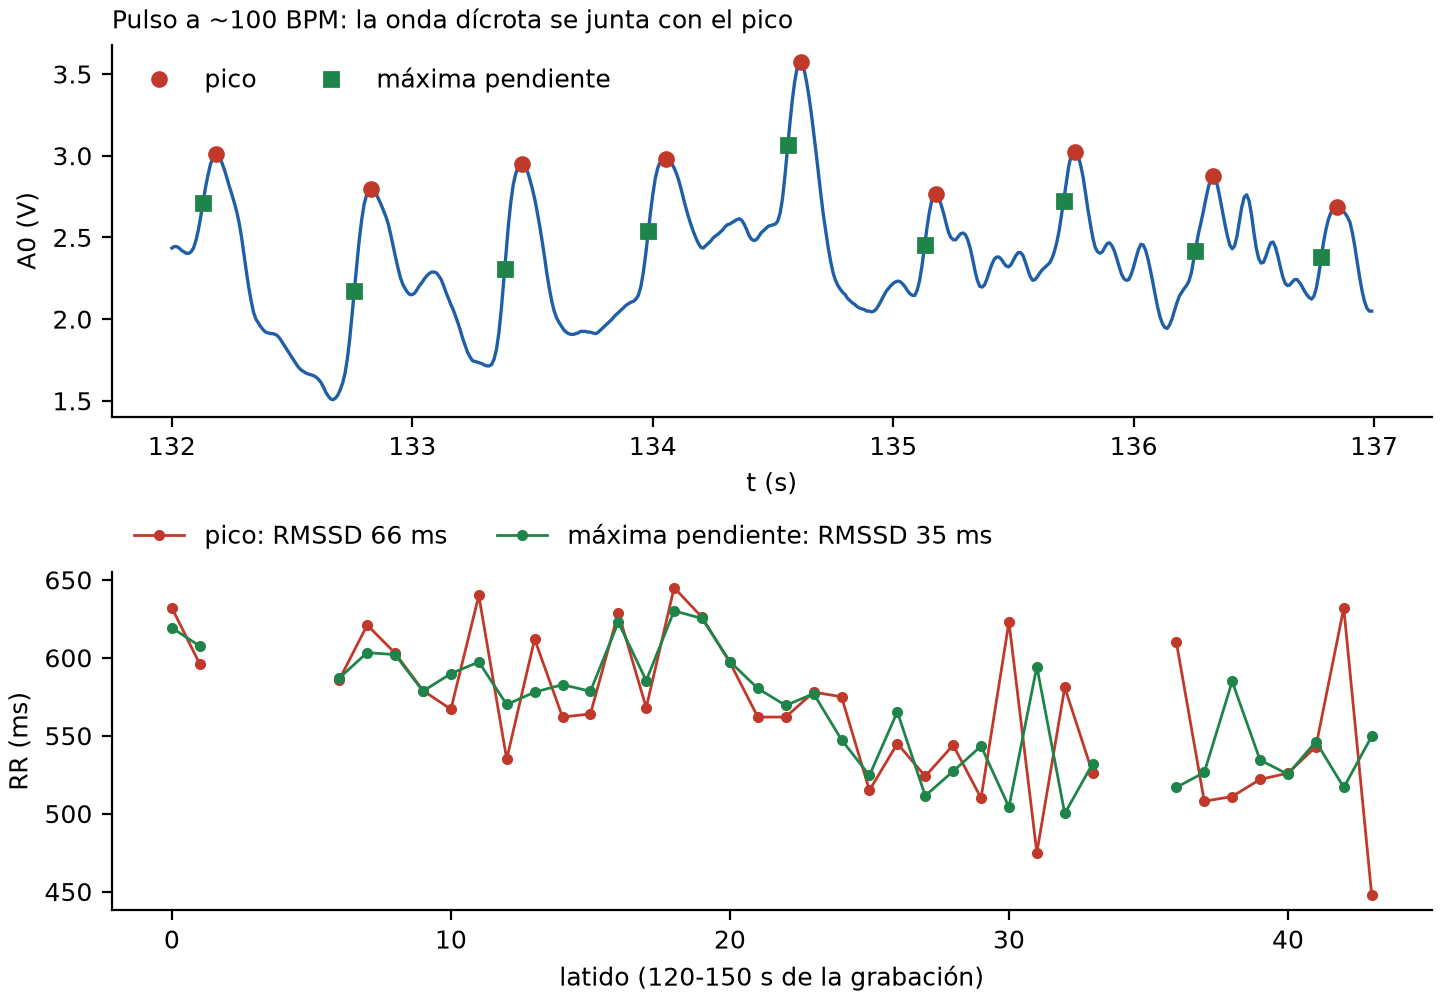
\includegraphics[width=0.88\textwidth]{informe_pico_pendiente.png}
\caption{Arriba: pulso a $\approx\qty{100}{BPM}$ con el instante de cada latido según el pico y
según la máxima pendiente. Abajo: RR de 30 s con cada método; los huecos son RR rechazados.}
\label{fig:fiducial}
\end{figure}

\textbf{2. Cambios bruscos de amplitud.} Al cambiar la presión del dedo, la amplitud cayó en
un caso de \qty{300}{LSB} a \qty{60}{LSB}. El umbral, adaptado latido a latido, quedó por
encima de los latidos pequeños y se perdieron 12 latidos en \qty{8.5}{s}. Ahora, si pasan 1,5
RR medios sin latido, el pico medio decae hacia el valle con $\tau = \qty{1}{s}$ y el umbral
alcanza los latidos pequeños sin esperar al reaprendizaje.

\textbf{3. Refractario con tope.} Un latido perdido da un RR doble que alarga el refractario
adaptativo. En una grabación eso tapaba el latido siguiente, y el detector se quedaba
enganchado contando la mitad de los latidos. La onda dícrota llega $\approx\qty{300}{ms}$
después del pico sea cual sea el ritmo, así que basta con limitar el refractario a
\qty{500}{ms}.

\subsection{BPM y HRV (M6)}

\begin{itemize}[leftmargin=1.2em,itemsep=2pt,topsep=2pt]
  \item \textbf{Rechazo de artefactos.} Un solo RR erróneo dispara el RMSSD: un latido perdido
        da un RR doble (+100\,\%) y uno de más lo parte (-50\,\%). Se descarta un RR fuera de
        \qtyrange{300}{2000}{ms} o que se aleje más de un \textbf{30\,\%} del último válido.
        El plan proponía un 20\,\%, pero en las grabaciones reales la arritmia respiratoria
        cambia el RR hasta un 25,5\,\% de un latido al siguiente: con 20\,\% se rechazaban 17
        RR buenos de 64; con 30\,\%, solo los 5 artefactos reales. Comparar con la mediana de
        los últimos 5 RR es peor: cuando el ritmo sube o baja varios latidos seguidos la
        mediana se queda atrás (hasta un 42\,\%).
  \item Sin referencia (al arrancar), el primer RR solo se acepta si coincide (\qty{\pm 30}{\percent})
        con el siguiente: si no, un primer RR malo se convertiría en referencia y haría
        rechazar los buenos. Con 5 rechazos seguidos se reinicia la referencia.
  \item \textbf{Ventana de 30 RR válidos} ($\approx\qty{30}{s}$), publicada a partir de 10 RR.
        En el RMSSD solo cuentan las diferencias entre RR realmente seguidos: si entre dos
        válidos hubo uno rechazado, esa diferencia no se usa. BPM con los últimos 8 RR
        válidos.
  \item \textbf{Aritmética entera exacta}: varianza
        $s^2 = \left(N\sum RR^2 - (\sum RR)^2\right)/\left(N(N-1)\right)$ en
        \texttt{uint32\_t}. Con $N \le 30$ y $RR \le \qty{2000}{ms}$,
        $N\sum RR^2 \le 3{,}6\cdot 10^9 < 2^{32}$: no hay desbordamiento ni error de redondeo
        hasta la raíz final.
\end{itemize}

\subsection{Indicador de estado (M7)}

La HRV varía mucho entre personas, así que el estado se decide respecto a una línea base
personal. La \textbf{calibración} (botón del visor, orden \texttt{c} o pulsador en D2) dura
\qty{2}{min} en reposo con al menos 60 RR válidos: $HR_0$ es el pulso medio y
$\mathrm{RMSSD}_0$ se calcula con todas las diferencias contiguas del periodo, no solo con la
ventana de 30. La línea base se guarda en la EEPROM (6 bytes con una marca de validez): abrir
el puerto serie reinicia el Nano, y sin ella habría que recalibrar cada vez que se abre el
visor. El estado mostrado solo cambia si el nuevo se mantiene 10 latidos seguidos.

\begin{table}[H]
\centering\small
\caption{Reglas de clasificación.}
\label{tab:estado}
\begin{tabularx}{\textwidth}{lX}
\toprule
Estado & Condición \\
\midrule
Relajado & $\mathrm{RMSSD} \ge 1{,}15\,\mathrm{RMSSD}_0$ y $HR \le HR_0 + 5$ \\
Estrés (plan) & ($\mathrm{RMSSD} \le 0{,}70\,\mathrm{RMSSD}_0$ y $HR \ge HR_0 + 10$) o $\mathrm{RMSSD} \le 0{,}5\,\mathrm{RMSSD}_0$ \\
\textbf{Estrés (final)} & ($HR \ge HR_0 + 10$ y $\mathrm{RMSSD} \le 1{,}15\,\mathrm{RMSSD}_0$) o $HR \ge HR_0 + 15$ o $\mathrm{RMSSD} \le 0{,}5\,\mathrm{RMSSD}_0$ \\
Normal & en otro caso \\
\bottomrule
\end{tabularx}
\end{table}

La regla de estrés del plan suponía que el RMSSD baja con el estrés. En nuestras pruebas con
cálculo mental el pulso subió 12-\qty{18}{BPM}, pero el RMSSD se quedó en 25-\qty{32}{ms}
con $\mathrm{RMSSD}_0 = \qty{25}{ms}$: nunca llegó al 70\,\% y el indicador no marcaba estrés.
La regla final da prioridad al pulso: estrés si sube 10 BPM sin que aumente la HRV, o si sube
15 BPM en cualquier caso (Sección~\ref{sec:estado}).

\subsection{Protocolo serie}

\begin{table}[H]
\centering\small
\caption{Mensajes entre Arduino y PC (ASCII, una línea por mensaje, \qty{115200}{baud}).}
\label{tab:protocolo}
\begin{tabularx}{\textwidth}{llX}
\toprule
Sentido & Formato & Significado \\
\midrule
Ard $\to$ PC & \texttt{S,<t>,<adc>} & Señal filtrada a \qty{100}{Hz} \\
Ard $\to$ PC & \texttt{B,<t>,<rr>,<res>,<bpm>,<rmssd>,<sdnn>,<est>} & Latido: instante y RR (ms), resultado del rechazo (0 válido, 1 sin RR, 2 fuera de rango, 3 artefacto), métricas y estado (0 sin calibrar, 1 calibrando, 2 relajado, 3 normal, 4 estrés) \\
Ard $\to$ PC & \texttt{I,<texto>} & Arranque, línea base, calibración, estadísticas cada \qty{5}{s} \\
PC $\to$ Ard & \texttt{c}, \texttt{r} & Calibrar; reiniciar detector y HRV \\
PC $\to$ Ard & \texttt{b<hr0>,<rmssd0>} & Cargar la línea base de un perfil (en décimas) \\
PC $\to$ Ard & \texttt{o} & Olvidar la línea base (vuelve a ``sin calibrar'') \\
\bottomrule
\end{tabularx}
\end{table}

% ======================================================================
\section{Software en el PC}

\textbf{Visor} (\texttt{pc/visor.py}, Tkinter con matplotlib embebido). Un hilo lee el puerto
serie y deja las líneas en una cola; la interfaz las procesa y se redibuja cada
\qty{40}{ms}. Redibujar la figura entera daba solo 6 fps. Los ejes están en tiempo relativo
(0 = ahora) y no cambian de un frame a otro, así que se guarda el fondo una vez y solo se
redibujan las curvas (\emph{blitting}). Además, el periodo descuenta lo que tarda cada frame.
Resultado: 20-\qty{25}{fps} con retraso estable, también reproduciendo grabaciones a 5×. Tiene
dos modos:
\begin{itemize}[leftmargin=1.2em,itemsep=2pt,topsep=2pt]
  \item \textbf{Test} (Figura~\ref{fig:visor}): onda con los latidos marcados, tacograma de
        \qty{60}{s} con los RR rechazados en rojo, métricas, fps y retraso. Graba siempre en
        CSV y permite marcar el inicio de cada fase de una prueba con la barra espaciadora.
  \item \textbf{Producción} (Figura~\ref{fig:produccion}): pantalla oscura y limpia para
        demostraciones y vídeos. Muestra el pulso (con un corazón que se enciende en cada
        latido), el estado, RMSSD y SDNN, cada uno con una explicación breve para quien no
        conoce los términos, y la onda al estilo de un monitor, que toma el color del estado.
        Sin dedo la onda es una línea recta: el autoescalado tiene un rango mínimo de
        \qty{1}{V} para no ampliar el bit de ruido del ADC. Todo escala con la ventana.
\end{itemize}
En ambos, \textbf{Calibrar} pide un nombre y guarda la línea base como perfil
(\texttt{datos/perfiles.json}); al elegir un perfil se envía al Nano. Así varias personas
pueden usar el pulsómetro sin recalibrar. ``Sin perfil'' hace que el Nano olvide la línea
base.

\begin{figure}[H]
\centering
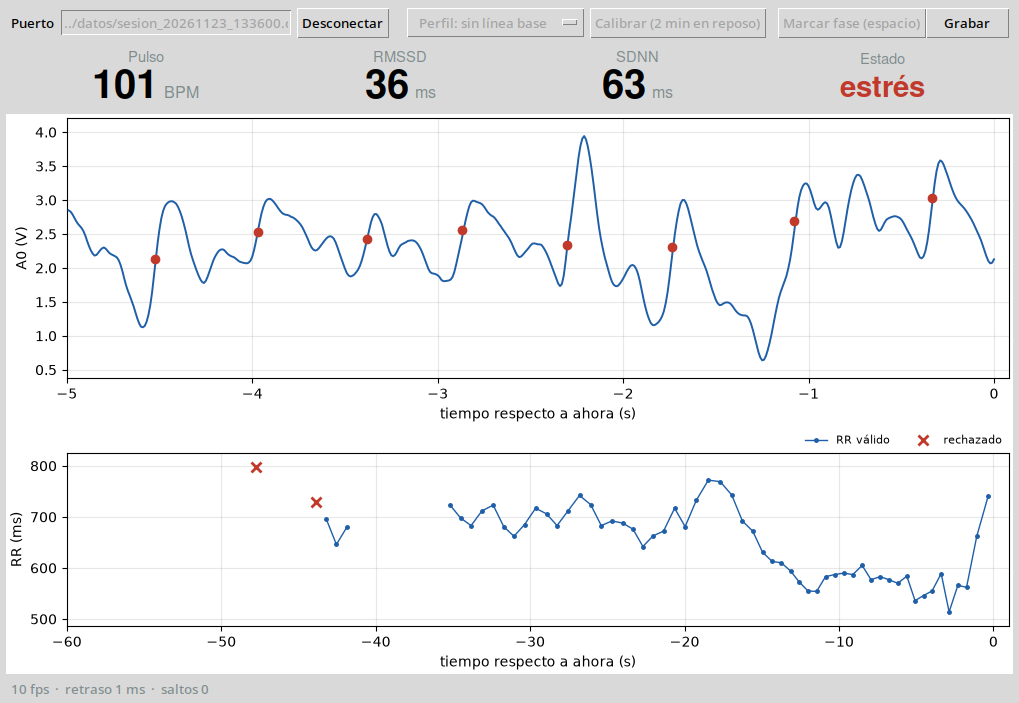
\includegraphics[width=0.8\textwidth]{m4_visor_test.png}
\caption{Visor en modo test durante la prueba de prensión: estado de estrés con
\qty{101}{BPM}.}
\label{fig:visor}
\end{figure}

\begin{figure}[H]
\centering
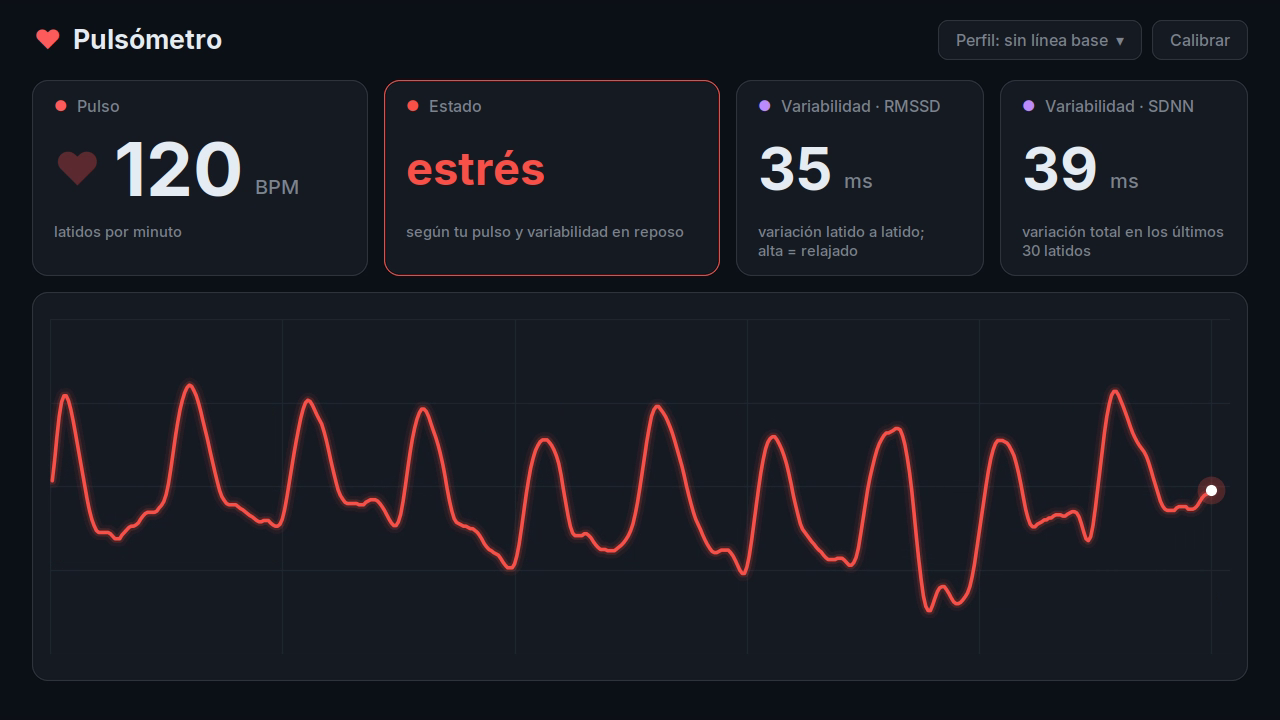
\includegraphics[width=0.8\textwidth]{m4_produccion.png}
\caption{Visor en modo producción durante una prueba de prensión: estado de estrés con
\qty{120}{BPM}.}
\label{fig:produccion}
\end{figure}

\textbf{Análisis} (\texttt{pc/analisis.py}): BPM, SDNN, RMSSD, pNN50 y diagrama de Poincaré de
una sesión completa. \textbf{Banco de pruebas} (\texttt{pc/test\_detector.cpp}): compila el
detector, la HRV y el estado del firmware en el PC y los ejecuta sobre cualquier grabación o
señal sintética (\texttt{pc/sintetica.py}), que reproduce la onda sistólica, la dícrota, el
ruido de red y la cuantización del ADC con RR conocidos. Cada cambio del firmware se
comprobó así con todas las grabaciones en segundos antes de cargarlo.

% ======================================================================
\section{Validación y resultados}

\subsection{Señales sintéticas}

\begin{table}[H]
\centering\small
\caption{Firmware final sobre señales sintéticas a \qty{500}{Hz} (ventana de 30 RR).}
\label{tab:sintetica}
\begin{tabularx}{\textwidth}{>{\raggedright\arraybackslash}X>{\raggedright\arraybackslash}X>{\raggedright\arraybackslash}X}
\toprule
Caso & Esperado & Medido \\
\midrule
60, 72 y \qty{120}{BPM} constantes & BPM exacto, RMSSD $\approx 0$ & 60,0 / 72,0 / 120,0 BPM; RMSSD 3,4-\qty{3.8}{ms} \\
RR alternando 800 y \qty{900}{ms} (prueba del plan) & RMSSD $100 \pm 2$, SDNN $50{,}9 \pm \qty{2}{ms}$ & \textbf{RMSSD 100,9 y SDNN \qty{51.4}{ms}} \\
Arritmia $RR = 800 + 60\sin(2\pi n/5)$ & RMSSD 49,0 y SDNN \qty{43.2}{ms} & 49,4 y \qty{43.6}{ms} \\
Arritmia con 3 latidos muy débiles & Los 3 RR dobles rechazados & 3 rechazados; 49,8 y \qty{43.8}{ms} \\
Protocolo de \qty{7}{min}: reposo, estrés, relajación & Estados en ese orden & Estrés a los \qty{17.5}{s} de empezar la fase de estrés; relajado en la relajación \\
\bottomrule
\end{tabularx}
\end{table}

El error de cada RR frente al valor real tiene media inferior a \qty{0.1}{ms} y valor eficaz
de $\approx\qty{2}{ms}$, de ahí el suelo de $\approx\qty{3.5}{ms}$ de RMSSD con ritmo
constante: pequeño frente a los 20-\qty{80}{ms} medidos en personas.

\subsection{Medidas con el dedo}

\textbf{Detección.} En \qty{60}{s} el Nano detectó 89 latidos, con RR entre 560 y
\qty{830}{ms}. Un buscador de picos independiente, escrito aparte sobre la misma señal,
cuenta también 89. Si el detector hubiera contado la onda dícrota habría RR de
$\approx\qty{300}{ms}$.

\textbf{BPM.} Se intentó validar con el conteo manual del pulso en el cuello y en la muñeca
durante \qty{60}{s}, pero las cuentas se desviaban hasta 13 latidos de la señal, en ambos
sentidos: no es una referencia válida para \qty{\pm 2}{BPM}. Frente a una aplicación de
móvil que mide el pulso con la cámara, el Nano dio \qty{77.6}{BPM} y la aplicación
\qty{79}{BPM}: error de \qty{1.4}{BPM}, dentro del criterio. La aplicación no es un instrumento
calibrado; con un pulsioxímetro la validación sería más sólida.

\textbf{HRV en reposo} (Figura~\ref{fig:hrv}): 53 latidos, 0 rechazados, \qty{80.2}{BPM},
SDNN \qty{60}{ms}, RMSSD \qty{32}{ms}, pNN50 13,5\,\%. El tacograma oscila entre 590 y
\qty{830}{ms} con un periodo de unos \qty{10}{s}: la arritmia sinusal respiratoria. En el
diagrama de Poincaré $SD2 \gg SD1$ ($81$ frente a \qty{23}{ms}), porque domina esa oscilación
lenta sobre la variación latido a latido. Valores normales para un adulto joven en
reposo~[3].

\begin{figure}[H]
\centering
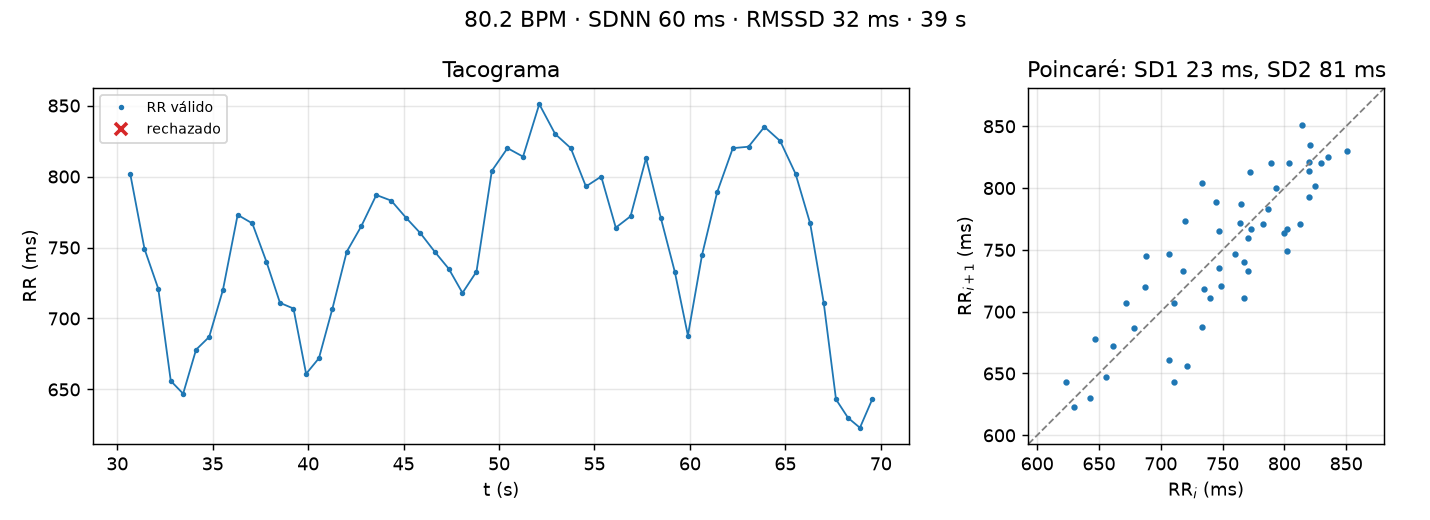
\includegraphics[width=0.9\textwidth]{m6_hrv_nano_1.png}
\caption{Sesión en reposo registrada con el Nano: tacograma y diagrama de Poincaré.}
\label{fig:hrv}
\end{figure}

\subsection{Indicador de estado}
\label{sec:estado}

\textbf{Calibración}: \qty{2}{min}, 164 RR con un solo rechazo. Línea base: $HR_0 =
\qty{82.8}{BPM}$, $\mathrm{RMSSD}_0 = \qty{25.0}{ms}$.

\textbf{Cálculo mental} (restar 7 desde 1000 durante 2-\qty{3}{min}): el pulso subió a 95-\qty{106}{BPM},
pero el RMSSD no bajó de \qty{25}{ms}. Con la regla del plan no se marcó estrés en ningún
momento. Además, hacer las restas en voz baja cambia la respiración, y con ella el RMSSD.

\textbf{Prueba rápida con prensión} (Figura~\ref{fig:prension}): unos \qty{20}{s} de reposo,
unos \qty{30}{s} apretando fuerte con la mano libre y respiración lenta (5\,s inspirando y 5\,s
espirando), con las fases marcadas en el visor. La prensión isométrica sube el pulso en pocos
segundos y es mucho más repetible que el cálculo mental. Resultado con la regla final:
\begin{itemize}[leftmargin=1.2em,itemsep=2pt,topsep=2pt]
  \item Reposo (85-\qty{88}{BPM}): normal.
  \item Prensión: el pulso sube a 103-\qty{107}{BPM} y el estado pasa a \textbf{estrés}
        \qty{10}{s} después de empezar (8 RR del promedio más 10 latidos de histéresis).
        Al cansarse el brazo el pulso bajó a $\approx\qty{95}{BPM}$ y el estado volvió a
        normal antes de terminar la fase.
  \item Respiración lenta: el pulso baja a 73-\qty{77}{BPM}, el RMSSD sube hasta
        \qty{80}{ms} y el estado pasa a \textbf{relajado}.
\end{itemize}

\begin{figure}[H]
\centering
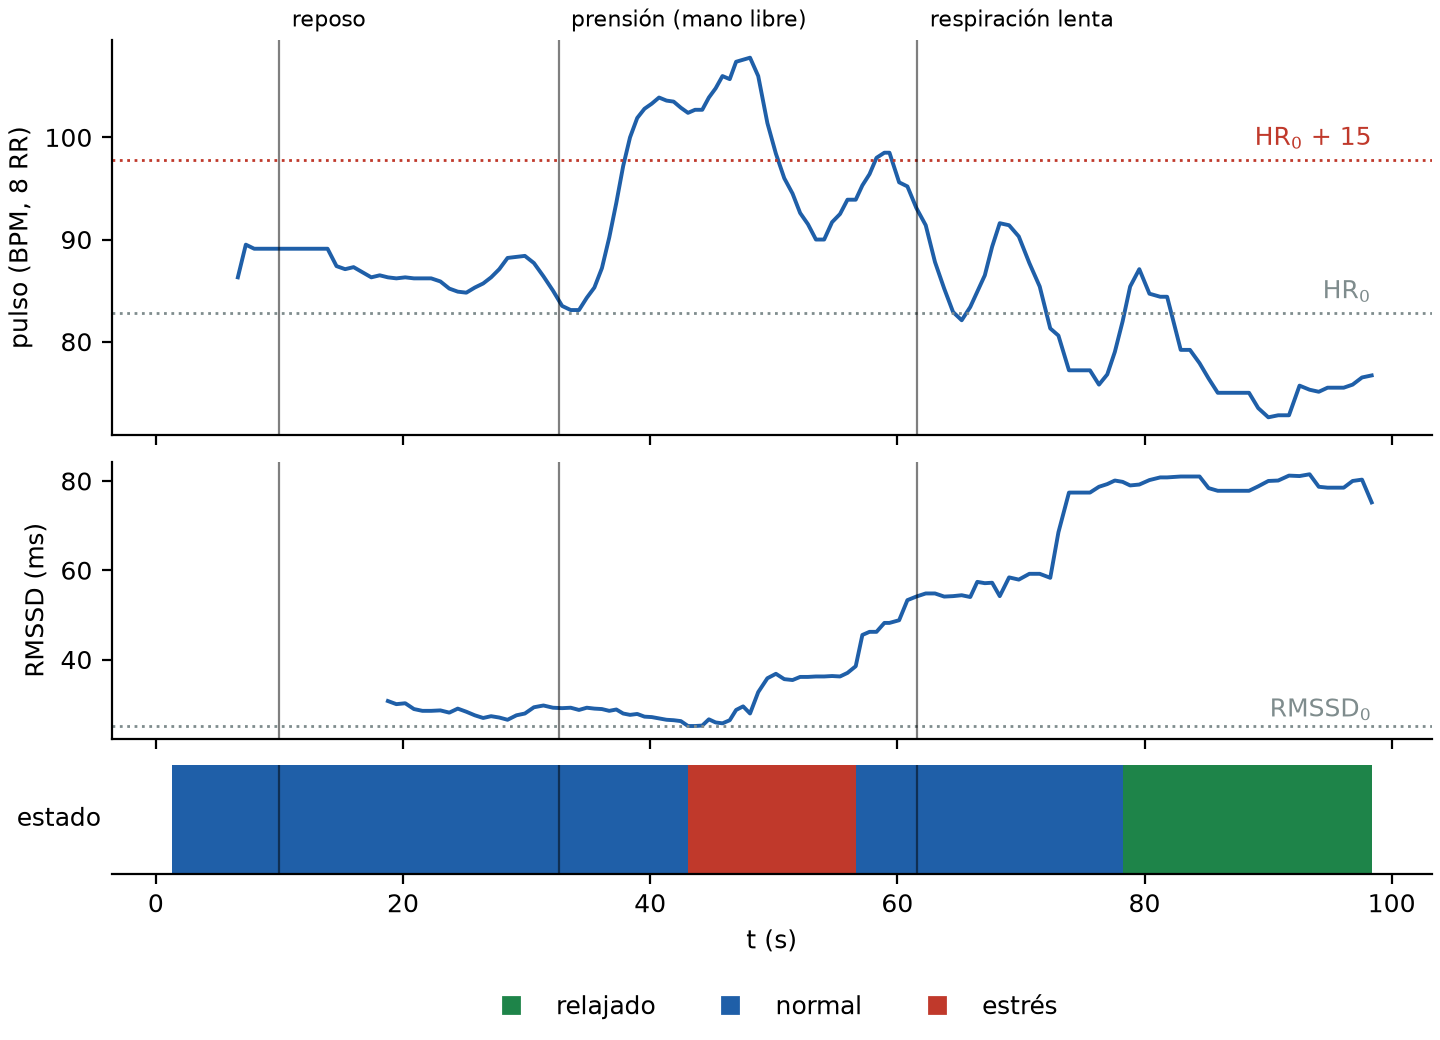
\includegraphics[width=0.88\textwidth]{informe_prension.png}
\caption{Prueba rápida de estado: pulso (media de 8 RR), RMSSD y estado mostrado por el Nano.
Las líneas verticales son las marcas de fase del visor.}
\label{fig:prension}
\end{figure}

\textbf{Segunda sesión, con dos personas.} Al día siguiente se repitió con el visor en modo
producción, grabando la pantalla:
\begin{itemize}[leftmargin=1.2em,itemsep=2pt,topsep=2pt]
  \item \textbf{Sin calibrar} (orden \texttt{o}): el visor muestra pulso, RMSSD y SDNN
        (\qty{92}{BPM} de media, 124 de 127 latidos válidos) y el estado ``sin calibrar'': sin
        línea base no hay con qué comparar.
  \item \textbf{Línea base del día anterior}: el reposo de ese día (88-\qty{97}{BPM}) quedaba
        cerca de $HR_0 + 15 = \qty{98}{BPM}$ y cualquier subida marcaba estrés.
  \item \textbf{Calibrando ese día} (Figura~\ref{fig:estadosvideo}): normal en reposo,
        \textbf{estrés} al apretar el puño (112-\qty{121}{BPM}), normal unos \qty{25}{s}
        después de soltar y \textbf{relajado} al relajarse (RMSSD 30-\qty{40}{ms}).
  \item \textbf{Segunda persona}: con su perfil el estado pasó de normal a \textbf{estrés}
        cuando el pulso subió a 91-\qty{102}{BPM} y siguió en estrés mientras su RMSSD estuvo
        por debajo de la mitad del de reposo. No llegó a relajado: su reposo ya era muy
        tranquilo y relajado exige $\mathrm{RMSSD} \ge \qty{80}{ms}$ sostenido.
\end{itemize}

\begin{table}[H]
\centering\small
\caption{Líneas base de calibración.}
\label{tab:lineasbase}
\begin{tabular}{lcc}
\toprule
 & $HR_0$ (BPM) & $\mathrm{RMSSD}_0$ (ms) \\
\midrule
Persona 1, día 1 & 82,8 & 25,0 \\
Persona 1, día 2 & 91,0 & 27,8 \\
Persona 2, día 2 & 65,9 & 69,2 \\
\bottomrule
\end{tabular}
\end{table}

La Tabla~\ref{tab:lineasbase} justifica la línea base personal: con umbrales absolutos, una
persona saldría casi siempre en estrés y la otra casi siempre relajada. Y la misma persona
cambia de un día a otro, así que conviene calibrar al empezar cada sesión.

\begin{figure}[H]
\centering
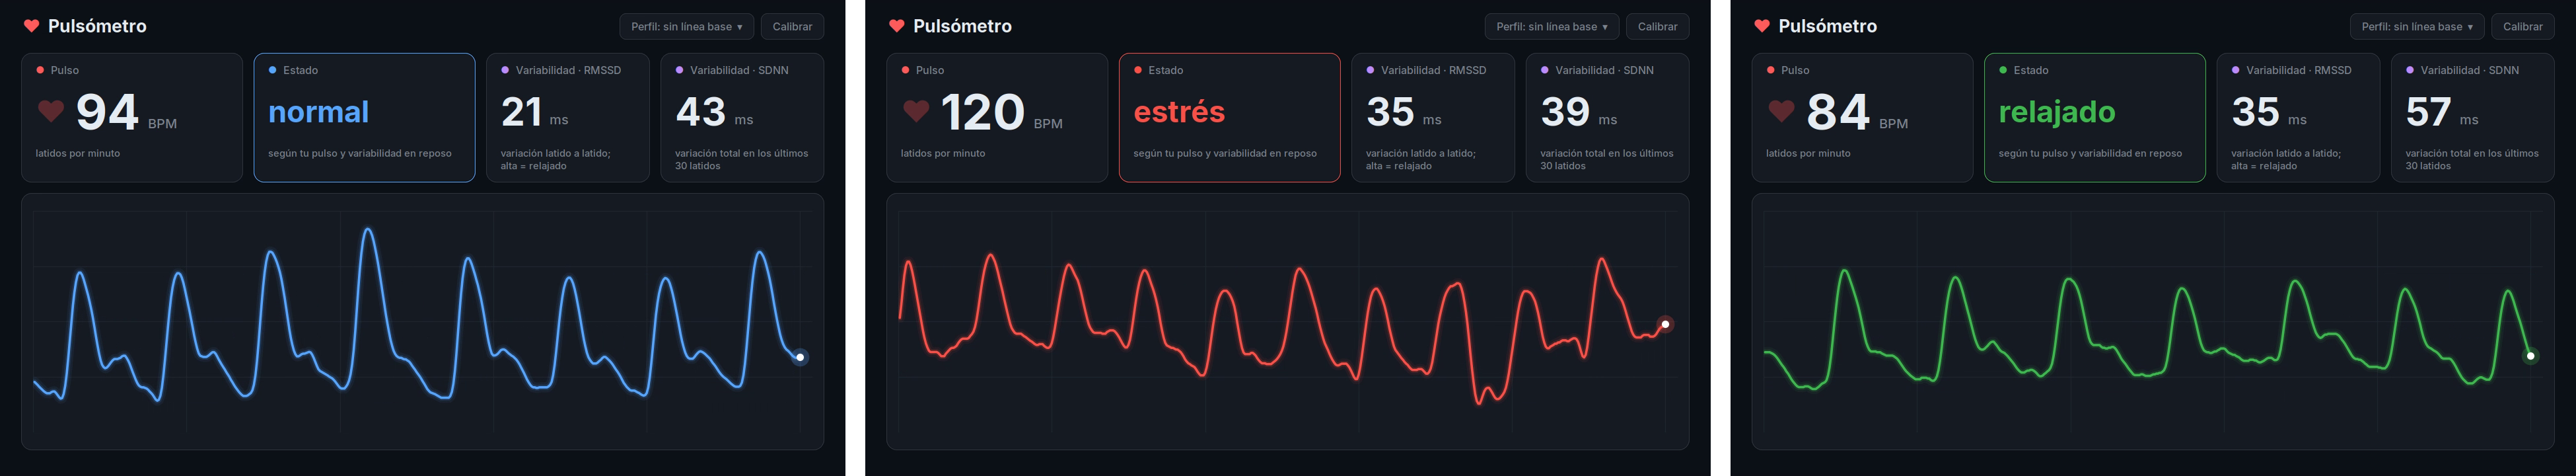
\includegraphics[width=\textwidth]{informe_estados_video.png}
\caption{Fotogramas del vídeo de la prueba con la línea base del día: normal en reposo,
estrés al apretar el puño y relajado al final. La onda toma el color del estado.}
\label{fig:estadosvideo}
\end{figure}

\textbf{Limitaciones.} El pulso en reposo varió entre 75 y \qty{92}{BPM} a lo largo de la
sesión, así que el umbral $HR_0 + 10$ produce alguna falsa alarma en reposo. En otra prueba
con respiración lenta el RMSSD apenas subió. A 6 respiraciones por minuto la oscilación de los
RR es lenta (unos \qty{\pm 60}{ms} cada $\approx 10$ latidos) y el RMSSD, que solo compara
latidos seguidos, la recoge mal; el SDNN de una ventana corta la recogería mejor. El
indicador es orientativo y no una medida clínica.

% ======================================================================
\Needspace{25\baselineskip}
\section{Problemas encontrados}

\begin{table}[H]
\centering\small
\caption{Principales problemas y cómo se resolvieron.}
\label{tab:problemas}
\begin{tabularx}{\textwidth}{>{\raggedright\arraybackslash}p{4.4cm}X}
\toprule
Problema & Causa y solución \\
\midrule
El sensor no era el previsto & LED blanco y LDR, no LED IR y fototransistor. Se identificó con el multímetro antes de montar (M0) y se diseñó el divisor para la máxima sensibilidad. \\
Solo había TL082 & Alimentación a \qty{\pm 12}{V}, etapas referidas a GND y desplazamiento final al centro del ADC con protección. \\
Etapa 2 saturada y raíl negativo cayendo & Faltaba la resistencia de realimentación (lazo abierto). Se puso el potenciómetro. Las resistencias se miden sin alimentación. \\
$C_1$ equivocado & Se montó uno de \qty{10}{nF} en vez de \qty{10}{\micro\farad} ($f_c$ de \qty{340}{Hz}); se detectó midiendo los componentes. \\
La ganancia no subía & Potenciómetro mal conectado (seguía a $\approx \qty{0}{\ohm}$); se vio en la grabación y se corrigió. \\
Latidos dobles y pérdidas & La onda dícrota y la deriva: refractario adaptativo, amplitud relativa mínima y cruce de subida obligatorio. \\
20\,\% de rechazo demasiado estricto & La arritmia respiratoria real llega al 25,5\,\%: 30\,\%. \\
RMSSD disparado a ritmo alto & El pico baila cuando la dícrota se junta con él: latido en la máxima pendiente. \\
Latidos perdidos al cambiar la presión & Umbral con decaimiento tras 1,5 RR sin latido; refractario con tope de \qty{500}{ms}. \\
El indicador no marcaba estrés & En estas pruebas el estrés se ve en el pulso, no en el RMSSD: regla basada en el pulso. \\
Línea base de otro día & El pulso en reposo cambió 8 BPM de un día a otro: calibrar en cada sesión; perfiles con nombre y orden para olvidar la línea base. \\
Pruebas perdidas por no pulsar Grabar & El visor graba siempre, con marcas de fase. \\
Visor a 6 fps & Blitting y periodo de refresco compensado: 20-\qty{25}{fps}. \\
\bottomrule
\end{tabularx}
\end{table}

% ======================================================================
\section{Conclusiones y mejoras}

El sistema cumple los objetivos principales: adquiere la señal PPG a \qty{500}{Hz} sin
pérdidas, detecta cada latido con precisión de pocos milisegundos y calcula BPM, RMSSD y SDNN
en el propio Arduino, con un error de BPM de \qty{1.4}{BPM} frente a la referencia y los
valores esperados de HRV con señales de RR conocidos. Las dos ampliaciones funcionan: la onda
se ve en tiempo real a más de \qty{20}{fps}, y el indicador de estado responde con la
tendencia esperada en la prueba de prensión y en la respiración lenta.

Lo más instructivo fue la distancia entre el plan y la señal real. Tanto el sensor como el
amplificador eran distintos de lo previsto, y el umbral de artefactos, el instante del
latido y la regla de estrés tuvieron que cambiarse tras medir. Tener el firmware compilable en
el PC permitió comprobar cada cambio con todas las grabaciones antes de cargarlo.

\textbf{Mejoras posibles}:
\begin{itemize}[leftmargin=1.2em,itemsep=2pt,topsep=2pt]
  \item Validar el BPM con un pulsioxímetro y la HRV con un ECG simultáneo.
  \item Usar el SDNN corto o la amplitud de la oscilación respiratoria para detectar la
        relajación con respiración lenta, y ajustar los umbrales de estado con más personas.
  \item Funcionamiento autónomo con LCD y LED RGB (M8).
  \item Un operacional \emph{rail-to-rail} a \qty{5}{V} eliminaría la fuente de
        \qty{\pm 12}{V}, y un LED infrarrojo con fotodiodo sería más rápido que la LDR.
\end{itemize}

% ======================================================================
\section*{Referencias}
\addcontentsline{toc}{section}{Referencias}

\begin{enumerate}[leftmargin=1.6em,itemsep=2pt,topsep=2pt,label={[\arabic*]}]
  \item Task Force of the European Society of Cardiology and the North American Society of
        Pacing and Electrophysiology. \emph{Heart rate variability: standards of measurement,
        physiological interpretation and clinical use}. Circulation 93(5), 1043-1065, 1996.
  \item J. Allen. \emph{Photoplethysmography and its application in clinical physiological
        measurement}. Physiological Measurement 28(3), R1-R39, 2007.
  \item F. Shaffer, J. P. Ginsberg. \emph{An overview of heart rate variability metrics and
        norms}. Frontiers in Public Health 5:258, 2017.
  \item M. L. Munoz et al. \emph{Validity of (ultra-)short recordings for heart rate
        variability measurements}. PLoS ONE 10(9): e0138921, 2015.
  \item A. Schäfer, J. Vagedes. \emph{How accurate is pulse rate variability as an estimate of
        heart rate variability?} International Journal of Cardiology 166(1), 15-29, 2013.
  \item Microchip. \emph{ATmega328P datasheet} (temporizadores, ADC, interrupciones).
  \item Texas Instruments. \emph{TL08xx JFET-input operational amplifiers datasheet}.
  \item Material de la asignatura: Temas 8, 9 y 10; \emph{Arduino Python} y
        \emph{Tkinter Python} (información complementaria).
\end{enumerate}

\end{document}
